\documentclass[11pt]{article}

\usepackage[margin=1in]{geometry}
\usepackage[T1]{fontenc}
\usepackage{lmodern}
\usepackage{amsmath,amssymb,amsthm}
\usepackage{graphicx}
\usepackage{booktabs}
\usepackage{multirow}
\usepackage{array}
\usepackage{xcolor}
\usepackage{hyperref}
\usepackage{caption}
\usepackage{subcaption}
\usepackage{enumitem}
\usepackage{listings}
\usepackage{microtype}
\usepackage{float}
\usepackage{tikz}
\usetikzlibrary{arrows.meta,positioning,calc,decorations.pathreplacing,decorations.pathmorphing,angles,quotes}
\usepackage{tcolorbox}
\tcbuselibrary{breakable,skins}

\newtcolorbox{intuition}[1][]{
  enhanced,breakable,colback=blue!4,colframe=blue!45!black,
  title=Intuition,fonttitle=\bfseries,left=4pt,right=4pt,top=4pt,bottom=4pt,#1}
\newtcolorbox{pitfall}[1][]{
  enhanced,breakable,colback=red!3,colframe=red!55!black,
  title=Common pitfall,fonttitle=\bfseries,left=4pt,right=4pt,top=4pt,bottom=4pt,#1}
\newtcolorbox{recipe}[1][]{
  enhanced,breakable,colback=green!3,colframe=green!45!black,
  title=Recipe,fonttitle=\bfseries,left=4pt,right=4pt,top=4pt,bottom=4pt,#1}

\hypersetup{
  colorlinks=true,
  linkcolor=blue!50!black,
  citecolor=blue!50!black,
  urlcolor=blue!50!black
}

\graphicspath{{figures/}}

\lstset{
  basicstyle=\ttfamily\small,
  breaklines=true,
  frame=single,
  backgroundcolor=\color{gray!6},
  keywordstyle=\color{blue!60!black},
  commentstyle=\color{green!40!black},
  stringstyle=\color{red!50!black},
  showstringspaces=false,
  columns=fullflexible,
  keepspaces=true
}

\newcommand{\bx}{\mathbf{x}}
\newcommand{\bp}{\mathbf{p}}
\newcommand{\bq}{\mathbf{q}}
\newcommand{\bv}{\mathbf{v}}
\newcommand{\bu}{\mathbf{u}}
\newcommand{\bA}{\mathbf{A}}
\newcommand{\bB}{\mathbf{B}}
\newcommand{\bQ}{\mathbf{Q}}
\newcommand{\bR}{\mathbf{R}}

\title{\textbf{Chapter 5 Assignment}\\[4pt]
Highly-articulated Legged Robots}
\author{Zihao Liu\\[2pt]
Student ID: 220261979\\[2pt]
\texttt{213222647@seu.edu.cn}}
\date{October 2026}

\begin{document}
\maketitle

\begin{abstract}
This report covers Chapter 5 of the course.  Part~I comments on the two
textbook examples: the ZMP planner (Example~5.1) and the LittleDog gait
optimization (Example~5.2).  The supplied notebooks were executed, the results
are interpreted with the centroidal-dynamics and ZMP theory of the chapter,
and the sensitivity to footstep timing, disturbances and gait parameters is
studied.  Part~II solves all exercises of Section~5.8: footstep planning via
mixed-integer quadratic programming (MIQP), the conceptual exercise on the
zero-moment point, and footstep planning via a graph of convex sets (GCS).
Both programming exercises pass their autograders with $16/16$ and $16/16$.
The complete Python code and the executed notebooks accompany the submission;
the most important code is reproduced in the appendix.
\end{abstract}

\tableofcontents
\newpage

%=====================================================================
\section{Overview and Reproducibility}
%=====================================================================

The assignment consists of:
\begin{itemize}[leftmargin=1.5em]
  \item \textbf{Examples} (code supplied; run and comment): Example~5.1
        (\texttt{ZmpPlanner}) and Example~5.2 (LittleDog gait optimization).
  \item \textbf{Section 5.8} (all exercises): MIQP footstep planning, the
        zero-moment-point exercise, and GCS footstep planning.
\end{itemize}

\begin{sloppypar}
All simulations use Drake 1.58.0 and the \texttt{underactuated} package
2026.9.8 in \texttt{/Users/leo/venvs/drake/bin/python} (NumPy 2.5.4,
SciPy 1.18.1, Matplotlib 3.11.2).  SNOPT is available in this Drake build and
is used both for the LittleDog trajectory optimization and for the GCS
shortest-path convex relaxation.  The exercise notebooks were executed
headlessly with \texttt{COLAB\_TESTING=1}, which prevents interactive
visualizers from blocking.  The LittleDog notebook was executed \emph{without}
that flag, because \texttt{running\_as\_notebook} must be true for SNOPT to be
allowed its full iteration budget; the complete optimization takes
$8.3$~s.
\end{sloppypar}

\begin{center}
\begin{tabular}{ll}
\toprule
Contents & Location \\
\midrule
Example notebooks & \texttt{Ch-5/Ch.5-examples/Exp5'1-*.ipynb}, \\
 & \texttt{Exp5'2-*.ipynb} \\
Section 5.8 notebooks & \texttt{Exp5'8-footstep-planning.ipynb}, \\
 & \texttt{Exp5'8-footstep-planning-gcs.ipynb} \\
Analysis scripts and figures & \texttt{Ch-5/exp5\_analysis/} \\
This report & \texttt{Ch-5/Ch5\_Assignment\_Report/} \\
\bottomrule
\end{tabular}
\end{center}

The autograder results are
\begin{center}
\texttt{MIQP footstep planning: 16/16.}\qquad
\texttt{GCS footstep planning: 16/16.}
\end{center}

\subsection*{How to read this report}

The report has three layers: \emph{models}, \emph{optimization} and
\emph{interpretation}.  If an equation looks dense, read the \textbf{Intuition}
boxes first: they give the physical picture without algebra.  The
\textbf{Recipe} boxes summarise a reusable procedure, and the
\textbf{Common pitfall} boxes point out the mistakes that are easy to make.

\begin{center}
\small
\begin{tabular}{p{0.16\textwidth}p{0.42\textwidth}p{0.34\textwidth}}
\toprule
Part & What is done & What to look for \\
\midrule
Example 5.1 & LIPM + \texttt{ZmpPlanner} & CoM lags the ZMP; timing changes
sway; feedback rejects pushes \\
Example 5.2 & LittleDog trajectory optimization & contact schedule; CoM and
angular-momentum constraints; gait snapshots \\
Section 5.8 (MIQP) & Big-M footstep planning & one stone per foot; step-span
limit; lateral detour \\
Section 5.8 (ZMP) & Foot/leg/bob analysis & ZMP line of action; heel lift;
actuated posture range \\
Section 5.8 (GCS) & Shortest path in a graph of convex sets & copies of
stones; edge constraints; LP relaxation \\
\bottomrule
\end{tabular}
\end{center}

\begin{intuition}[breakable=false,title={The big picture in five sentences}]
A highly articulated robot that stands on flat ground can be planned from the
outside in: first choose footsteps, then choose a CoM trajectory whose
zero-moment point stays inside the support polygon, and finally realize that
CoM trajectory with the whole body.  The CoM equations are exact for the full
multibody system; the only approximation is the set of contact forces the
robot can produce.  Footstep planning is a combinatorial problem, solved
either by branch and bound over binaries (MIQP) or by a shortest path in a
graph of convex sets (GCS).  The ZMP is the bridge between the two layers: it
turns a contact constraint into a constraint on CoM acceleration.
\end{intuition}

\begin{center}
\small
\begin{tabular}{ll}
\toprule
Symbol & Meaning \\
\midrule
$\bp_{cm}=(x,y,z)$ & center of mass position \\
$\bp_{cp}$, $\bp_{zmp}$ & center of pressure / zero-moment point \\
$m$ & total mass \\
$z$ & constant CoM height in the LIPM \\
$\mathbf{f}_i$ & contact force at contact point $i$ \\
$\mu$ & friction coefficient \\
$d$ & step span (side of the reachable square) \\
$\delta_{t,i}$ & binary: foot at step $t$ is on stone $i$ \\
$N,L_1,L_2,h$ & exercise parameters (leg length, toe/heel offsets, ankle height) \\
\bottomrule
\end{tabular}
\end{center}

%=====================================================================
\section{Example 5.1: The ZMP Planner}
%=====================================================================

\subsection{Model: the linear inverted pendulum and the ZMP}

For a point mass at constant height $z$, the horizontal CoM dynamics are the
linear inverted pendulum model (LIPM)
\begin{equation}
\ddot{\mathbf{c}}=\frac{g}{z}\left(\mathbf{c}-\mathbf{y}\right),
\label{eq:lipm}
\end{equation}
where $\mathbf{c}=(x,y)$ is the CoM position and $\mathbf{y}$ is the
zero-moment point.  On flat ground the ZMP coincides with the center of
pressure (CoP), i.e.\ with the point where the resultant ground reaction acts.
Equation~\eqref{eq:lipm} is another way of writing the moment balance
\begin{equation}
\mathbf{y}=\mathbf{c}-\frac{z}{g}\ddot{\mathbf{c}} .
\label{eq:zmp}
\end{equation}
The ZMP must lie in the support polygon; for a single flat foot this is the
segment between heel and toe.

\begin{figure}[htbp]
\centering
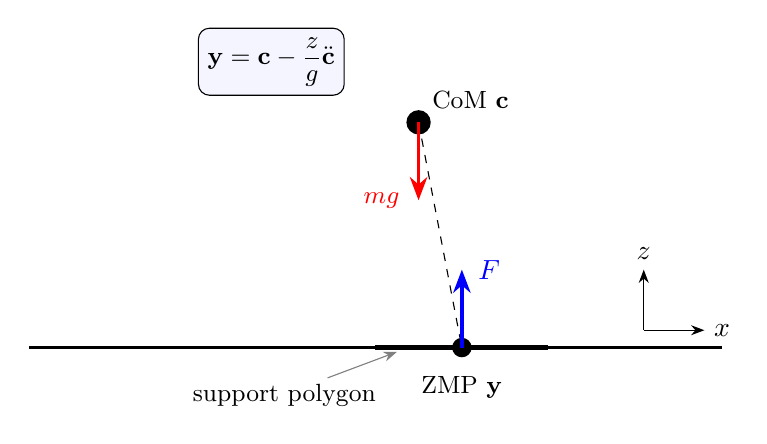
\begin{tikzpicture}[>=Stealth,scale=1.1]
  \draw[thick] (-2.8,0)--(5.2,0);
  \draw[ultra thick,black] (1.2,0)--(3.2,0);
  \node[align=center,font=\small] at (0.15,-0.55) {support polygon};
  \draw[->,gray] (0.65,-0.35)--(1.45,-0.05);
  \coordinate (C) at (1.7,2.6);
  \coordinate (Z) at (2.2,0);
  \fill (C) circle (4pt);
  \node[above right=2pt,font=\small] at (C) {CoM $\mathbf{c}$};
  \fill (Z) circle (3.2pt);
  \node[below=7pt,font=\small] at (Z) {ZMP $\mathbf{y}$};
  \draw[dashed] (C)--(Z);
  \draw[->,very thick,red] (C)--++(0,-0.9) node[left=3pt,font=\small] {$mg$};
  \draw[->,very thick,blue] (Z)--++(0,0.9) node[right=2pt] {$F$};
  \draw[->] (4.3,0.2)--++(0.7,0) node[right] {$x$};
  \draw[->] (4.3,0.2)--++(0,0.7) node[above] {$z$};
  \node[draw,rounded corners,fill=blue!4,font=\small] at (0.0,3.3)
       {$\mathbf{y}=\mathbf{c}-\dfrac{z}{g}\ddot{\mathbf{c}}$};
\end{tikzpicture}
\caption{The LIPM and the ZMP.  The ground reaction at the ZMP and gravity at
the CoM form a couple that produces the CoM acceleration.  Keeping the ZMP
inside the support polygon (the black segment under the foot) keeps the foot
flat.}
\label{fig:lipm_zmp}
\end{figure}

Drake's \texttt{ZmpPlanner} takes a desired ZMP trajectory
$\mathbf{y}_d(t)$ (a piecewise polynomial), an initial CoM state
$\bx_0=[\mathbf{c}_0;\dot{\mathbf{c}}_0]$ and the height $z$, and solves
\begin{equation}
\min_{\mathbf{y},\ddot{\mathbf{c}}}\;
\int_0^{t_f}\left[
\|\mathbf{y}(t)-\mathbf{y}_d(t)\|^2_{\bQ_y}
+\|\ddot{\mathbf{c}}(t)\|^2_{\bR}
\right]dt
+\bar{\bx}(t_f)^\top \mathbf{S}\,\bar{\bx}(t_f),
\label{eq:zmp_cost}
\end{equation}
subject to~\eqref{eq:zmp}, where $\bar{\bx}$ is the state relative to the final
ZMP and $\mathbf{S}$ is the infinite-horizon LQR cost-to-go of the same
dynamics.  The solution is a nominal CoM trajectory together with a
time-varying linear feedback policy
\begin{equation}
\ddot{\mathbf{c}}^*=\mathbf{K}(t)\left(\bx(t)-\bx_{\rm nom}(t)\right)
+\ddot{\mathbf{c}}_{\rm nom}(t).
\label{eq:zmp_policy}
\end{equation}
This is the important practical point: the planner does not only return a
trajectory, it returns a policy that rejects state perturbations.

\begin{recipe}[breakable=false,title={Building a ZMP plan from footsteps}]
\begin{enumerate}[leftmargin=1.4em,itemsep=2pt]
  \item Choose a footstep sequence $\bp_0,\bp_1,\dots$ and a timing
        (single-support and double-support durations).
  \item Build the desired ZMP as a piecewise-linear path between the foot
        centers: hold at each foot during single support, interpolate during
        double support.
  \item Call \texttt{ZmpPlanner.Plan(zmp\_traj, x0, height)}.
  \item Evaluate \texttt{get\_nominal\_com}, \texttt{get\_nominal\_comd} and
        \texttt{ComputeOptimalCoMdd}; use the latter as the feedback policy.
  \item Check that the realized ZMP $\mathbf{c}-(z/g)\ddot{\mathbf{c}}$ stays
        inside the support polygon and close to the desired one.
\end{enumerate}
\end{recipe}

\subsection{Nominal plan and timing sensitivity}

The supplied notebook was completed with a plotting and evaluation block.  The
footsteps are
\[
\text{footsteps}=[(0,-0.05),(0.5,0.05),(1,-0.05),(1.5,0.05),(2,-0.05),(2.5,0.05)],
\]
i.e.\ a 0.5~m stride with a 0.1~m lateral sway, and the CoM height is $z=1$~m.
The nominal timing is a 0.5~s double support and a 1.0~s single support.

\begin{figure}[htbp]
  \centering
  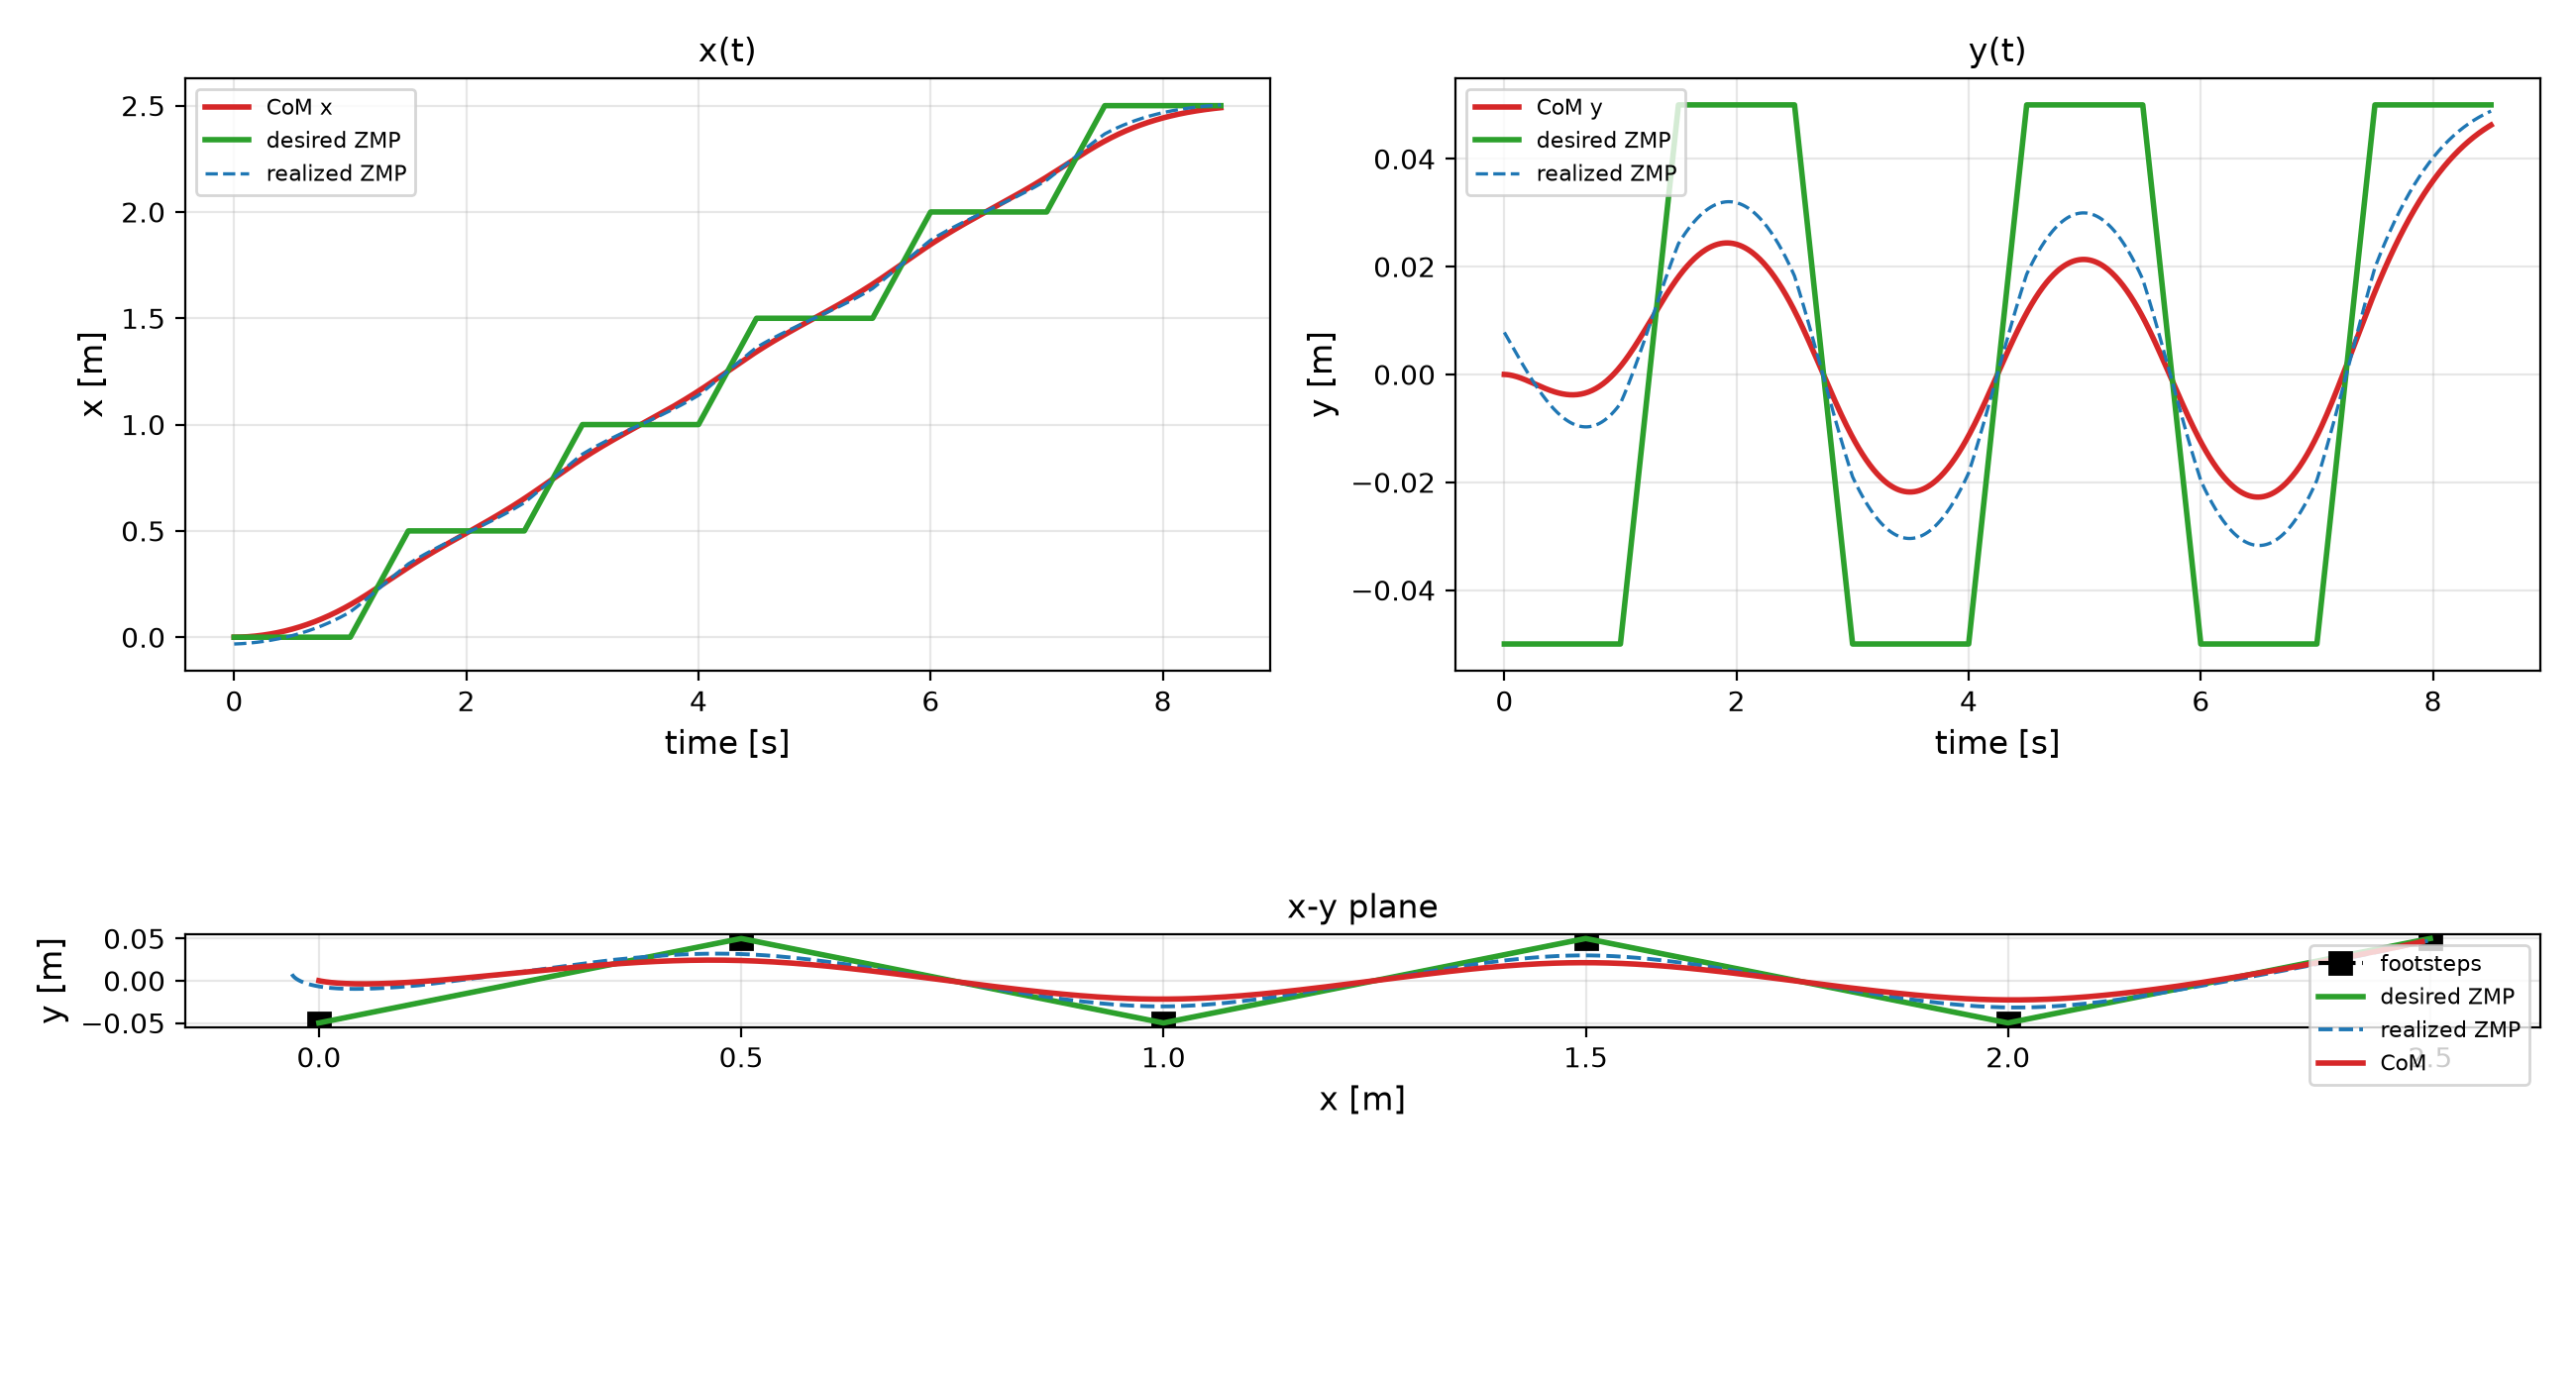
\includegraphics[width=0.98\textwidth]{fig5_1_zmp_plan.png}
  \caption{Example 5.1, nominal plan.  Top: CoM and realized/desired ZMP in
  $x(t)$ and $y(t)$.  Bottom: top view.  The realized ZMP is smoother than the
  commanded staircase because the quadratic cost~\eqref{eq:zmp_cost} trades
  ZMP tracking against CoM acceleration.}
  \label{fig:zmp_nominal}
\end{figure}

\begin{table}[H]
\centering
\caption{Example 5.1: nominal plan metrics.}
\begin{tabular}{ll}
\toprule
Quantity & Value \\
\midrule
Plan duration & 8.50 s \\
Peak lateral CoM excursion $\max_t|\mathrm{CoM}_y|$ & 46.3 mm \\
Maximum ZMP tracking error & 0.158 m \\
RMS ZMP tracking error & 0.078 m \\
Final CoM $x$ & 2.490 m (last footstep at 2.500 m) \\
\bottomrule
\end{tabular}
\end{table}

The CoM sway is only 4.6~cm although the footsteps alternate by 10~cm; the
finite Q/R weighting makes the CoM cut the corners of the ZMP staircase.  The
ZMP tracking error is not zero: with $\bQ_y=I$ and $\bR=0.1I$ the planner
prefers a smooth CoM acceleration and accepts a lag of up to 15.8~cm during
double support.  This is a useful reminder that a ``ZMP plan'' is an
optimal-trade-off plan, not a hard equality constraint.

\begin{table}[H]
\centering
\caption{Example 5.1: footstep-timing sensitivity (DS = double support,
SS = single support).}
\begin{tabular}{ccccc}
\toprule
DS [s] & SS [s] & duration [s] & peak $|\mathrm{CoM}_y|$ [m] &
max ZMP error [m] \\
\midrule
0.2 & 1.4 & 9.40 & 0.0490 & 0.204 \\
0.5 & 1.0 & 8.50 & 0.0463 & 0.158 \\
1.0 & 0.5 & 8.00 & 0.0411 & 0.095 \\
1.0 & 1.0 & 11.00 & 0.0485 & 0.101 \\
\bottomrule
\end{tabular}
\end{table}

\begin{figure}[htbp]
  \centering
  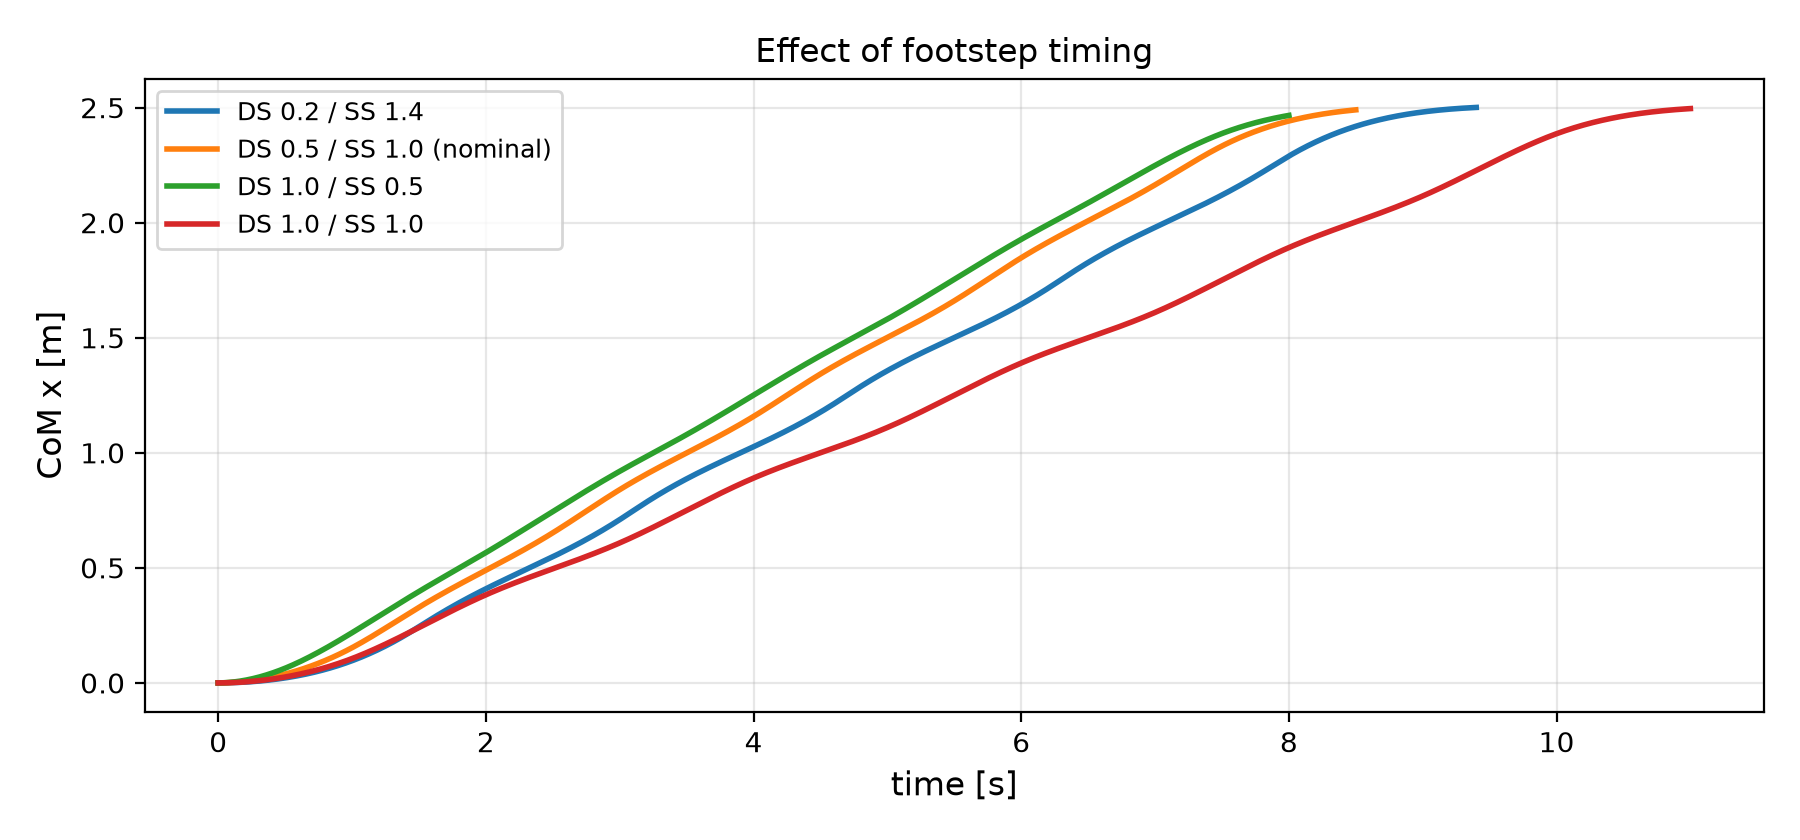
\includegraphics[width=0.78\textwidth]{fig5_2_zmp_timing.png}
  \caption{Example 5.1: CoM $x(t)$ for four footstep timings.  Longer single
  support means a longer plan and larger lateral sway; a long double support
  with a short single support gives the fastest walk in this set.}
  \label{fig:zmp_timing}
\end{figure}

\textbf{Comments.}  The single-support duration is the time the ZMP is held at
one foot; the double-support duration is the time it travels between feet.  A
long single support leaves the CoM on its own for longer, so the pendulum
falls farther laterally and the planner must use a larger sway.  A long double
support smooths the ZMP motion and reduces the tracking error, but it makes
the plan longer.  The fastest plan in the table (DS $=1.0$, SS $=0.5$) is also
the one with the smallest tracking error, because the ZMP moves quickly
between feet and then rests, which is easy for the LIPM to follow.

\subsection{The feedback policy rejects disturbances}

The planner's value function gives the policy~\eqref{eq:zmp_policy}.  We
simulated the LIPM in closed loop from four initial states: the nominal state,
a $+0.30$~m/s and a $-0.30$~m/s horizontal velocity perturbation, and a
$(5,3)$~cm CoM position offset.

\begin{table}[H]
\centering
\caption{Example 5.1: closed-loop response to initial-state perturbations.}
\begin{tabular}{lccc}
\toprule
Case & max $x$ deviation [m] & final $x$ deviation [m] &
final $y$ deviation [m] \\
\midrule
nominal & 0 & 0 & 0 \\
push $+0.30$ m/s in $x$ & 0.0709 & $1.2\times10^{-6}$ & 0 \\
push $-0.30$ m/s in $x$ & 0.0709 & $-1.2\times10^{-6}$ & 0 \\
CoM offset $(5,3)$ cm & 0.0500 & $8.5\times10^{-8}$ & $5.1\times10^{-8}$ \\
\bottomrule
\end{tabular}
\end{table}

\begin{figure}[htbp]
  \centering
  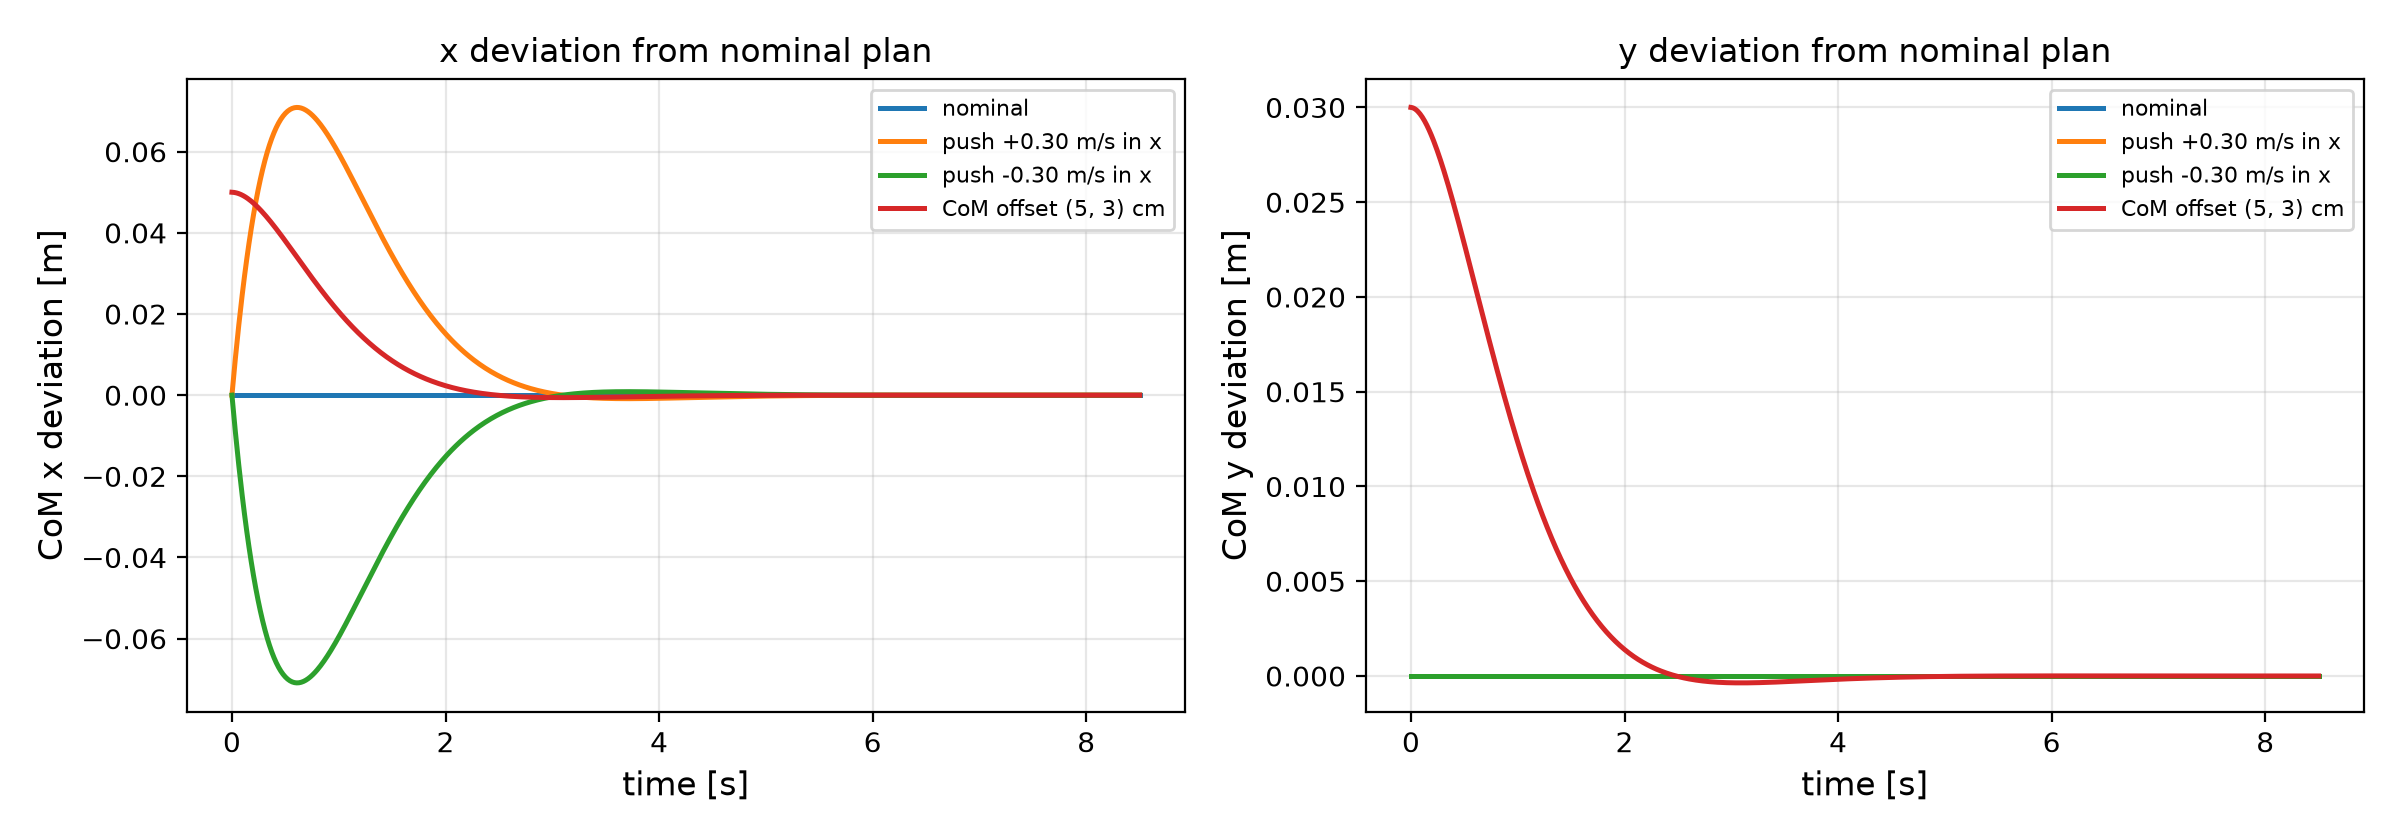
\includegraphics[width=0.9\textwidth]{fig5_3_zmp_feedback.png}
  \caption{Example 5.1: deviation from the nominal plan under initial-state
  perturbations.  The feedback policy removes a 0.30~m/s push within the
  8.5~s plan; the residual at the final time is at the level of integration
  error.}
  \label{fig:zmp_feedback}
\end{figure}

\begin{intuition}[breakable=false,title={Why a ZMP planner is a feedback controller}]
The LIPM is an unstable inverted pendulum: a small velocity error grows like
$\exp(t\sqrt{g/z})$.  The ZMP plan alone would diverge.  The value function of
the LQR problem, however, defines the optimal cost-to-go for every state, and
its gradient gives a linear feedback law.  Pushing the CoM forward makes the
policy move the ZMP forward, which decelerates the CoM.  In this sense the ZMP
trajectory is a feedforward term and the policy is the feedback term.
\end{intuition}

\begin{pitfall}[breakable=false,title={The ZMP is not the CoM}]
A common mistake is to draw the CoM path and call it the ZMP, or to assume the
ZMP must equal the CoM projection.  They coincide only when the CoM
acceleration is zero.  During walking the CoM is constantly accelerating, and
the ZMP leads or lags it by $(z/g)\ddot{\mathbf{c}}$.  In
Fig.~\ref{fig:zmp_nominal} the desired ZMP is a staircase while the CoM is a
smooth curve; the horizontal gap between them is exactly the acceleration
term.
\end{pitfall}

\textbf{Comments.}  The example makes the layering of Chapter~5 concrete: the
footstep sequence defines a ZMP trajectory, the ZMP trajectory defines a CoM
plan and a feedback policy, and a whole-body controller would then realize the
CoM plan with the joints.  The LIPM ignores the angular momentum about the
CoM; for slow walking this is a good approximation, but fast motions or arm
swing require the centroidal-dynamics formulation discussed in the chapter.

%=====================================================================
\section{Example 5.2: LittleDog Gait Optimization}
%=====================================================================

\subsection{Model and decision variables}

LittleDog is a small quadruped with a floating base and three joints per leg
(hip roll, hip pitch, knee): $n_q=7+12=19$ positions and $n_v=6+12=18$
velocities.  The optimization is a direct transcription with $N=21$ knot
points.  The decision variables are
\begin{itemize}[leftmargin=1.5em]
  \item the $N-1$ time steps $h_n>0$;
  \item the configurations $\bq_n\in\mathbb{R}^{19}$ and velocities
        $\bv_n\in\mathbb{R}^{18}$;
  \item the four contact forces $\mathbf{f}_{i,n}\in\mathbb{R}^3$ at the four
        feet;
  \item the CoM position/velocity/acceleration $\mathbf{c}_n,\dot{\mathbf{c}}_n,
        \ddot{\mathbf{c}}_n$;
  \item the centroidal angular momentum $\mathbf{H}_n$ and its rate
        $\dot{\mathbf{H}}_n$.
\end{itemize}

\subsection{Constraints and costs}

The transcription enforces:
\begin{align}
\bv_{n+1}-\bv_n &= h_n\dot{\bv}_n, &
\bq_{n+1}-\bq_n &= h_n\,\bB(\bq_n)\bv_n, \label{eq:little_dyn}\\
m\ddot{\mathbf{c}}_n &= \sum_{i=1}^{4}\mathbf{f}_{i,n}+m\mathbf{g}, &
\dot{\mathbf{H}}_n &= \sum_{i=1}^{4}
   (\bp_{i,n}-\mathbf{c}_n)\times\mathbf{f}_{i,n}, \label{eq:little_com}\\
\mathbf{c}_n &= \mathrm{CoM}(\bq_n), &
\mathbf{H}_n &= \mathbf{A}(\bq_n,\bv_n)\bv_n, \label{eq:little_centroidal}\\
|f_{i,n}^{x}|&\le\mu f_{i,n}^{z}, &
|f_{i,n}^{y}|&\le\mu f_{i,n}^{z}, \label{eq:little_friction}\\
0\le f_{i,n}^{z}&\le s_{i,n}\,4mg, \label{eq:little_normal}
\end{align}
where $s_{i,n}\in\{0,1\}$ is the prescribed stance schedule.  The kinematic
constraints force a stance foot to be on the ground ($z=0$) and not to move
between consecutive stance knots, and force a swing foot to have at least
1~cm clearance.  Joint position and velocity limits, unit quaternions and a
body-orientation constraint are imposed at every knot.  Periodic boundary
conditions are imposed on the half stride (the gait is laterally symmetric,
so a half stride plus a mirror reflection produces a full stride).

The cost is a quadratic running cost
\begin{equation}
\sum_{n=0}^{N-1}\left[
(\bq_n-\bq_{\rm home})^\top \bQ_q(\bq_n-\bq_{\rm home})
+\bv_n^\top \bQ_v\bv_n
\right],
\end{equation}
with larger weights on the hip-roll joints (to discourage splaying), plus the
implicit objective of finding any feasible gait.  The problem is solved with
SNOPT.

\begin{recipe}[breakable=false,title={Contact-implicit versus contact-scheduled transcription}]
\begin{enumerate}[leftmargin=1.4em,itemsep=2pt]
  \item Choose a contact schedule: a binary stance matrix $s_{i,n}$ for each
        foot and knot.
  \item Add contact forces only where $s_{i,n}=1$ (normal-force upper bound
        $s_{i,n}4mg$).
  \item Impose the centroidal dynamics~\eqref{eq:little_com} and the
        centroidal consistency~\eqref{eq:little_centroidal} at every knot.
  \item Impose full kinematics: stance foot fixed on the ground, swing foot
        above the ground, joint limits.
  \item Add periodicity and solve with a local nonlinear solver from a good
        initial guess (the home configuration).
\end{enumerate}
\end{recipe}

\subsection{Results}

The notebook solves the walking-trot schedule in 8.3~s and SNOPT reports
success.  The optimal cost is $419.76$.

\begin{table}[H]
\centering
\caption{Example 5.2: walking-trot solution metrics.}
\begin{tabular}{ll}
\toprule
Quantity & Value \\
\midrule
Gait & walking trot (lateral symmetry) \\
SNOPT status & success \\
Optimal cost & 419.76 \\
Solve time & 8.3 s \\
Half-stride duration & 0.34375 s \\
Full-stride duration & 0.6875 s \\
Stride length & 0.25 m \\
Effective speed & 0.364 m/s (requested 0.4 m/s) \\
CoM height range & 0.1309--0.1484 m \\
Maximum body pitch & 0.0189 rad \\
Maximum foot clearance & 11.9 mm \\
Maximum normal force & 74.8 N (back right) \\
\bottomrule
\end{tabular}
\end{table}

The effective speed is slightly below the requested 0.4~m/s because the
optimizer chose half-stride durations at the upper end of the allowed window
($1.1T$, with $T=0.3125$~s).  This is consistent with the cost: the squared
joint velocities penalize fast motion, so the solver stretches the stride in
time until it hits the bound.

\begin{figure}[htbp]
  \centering
  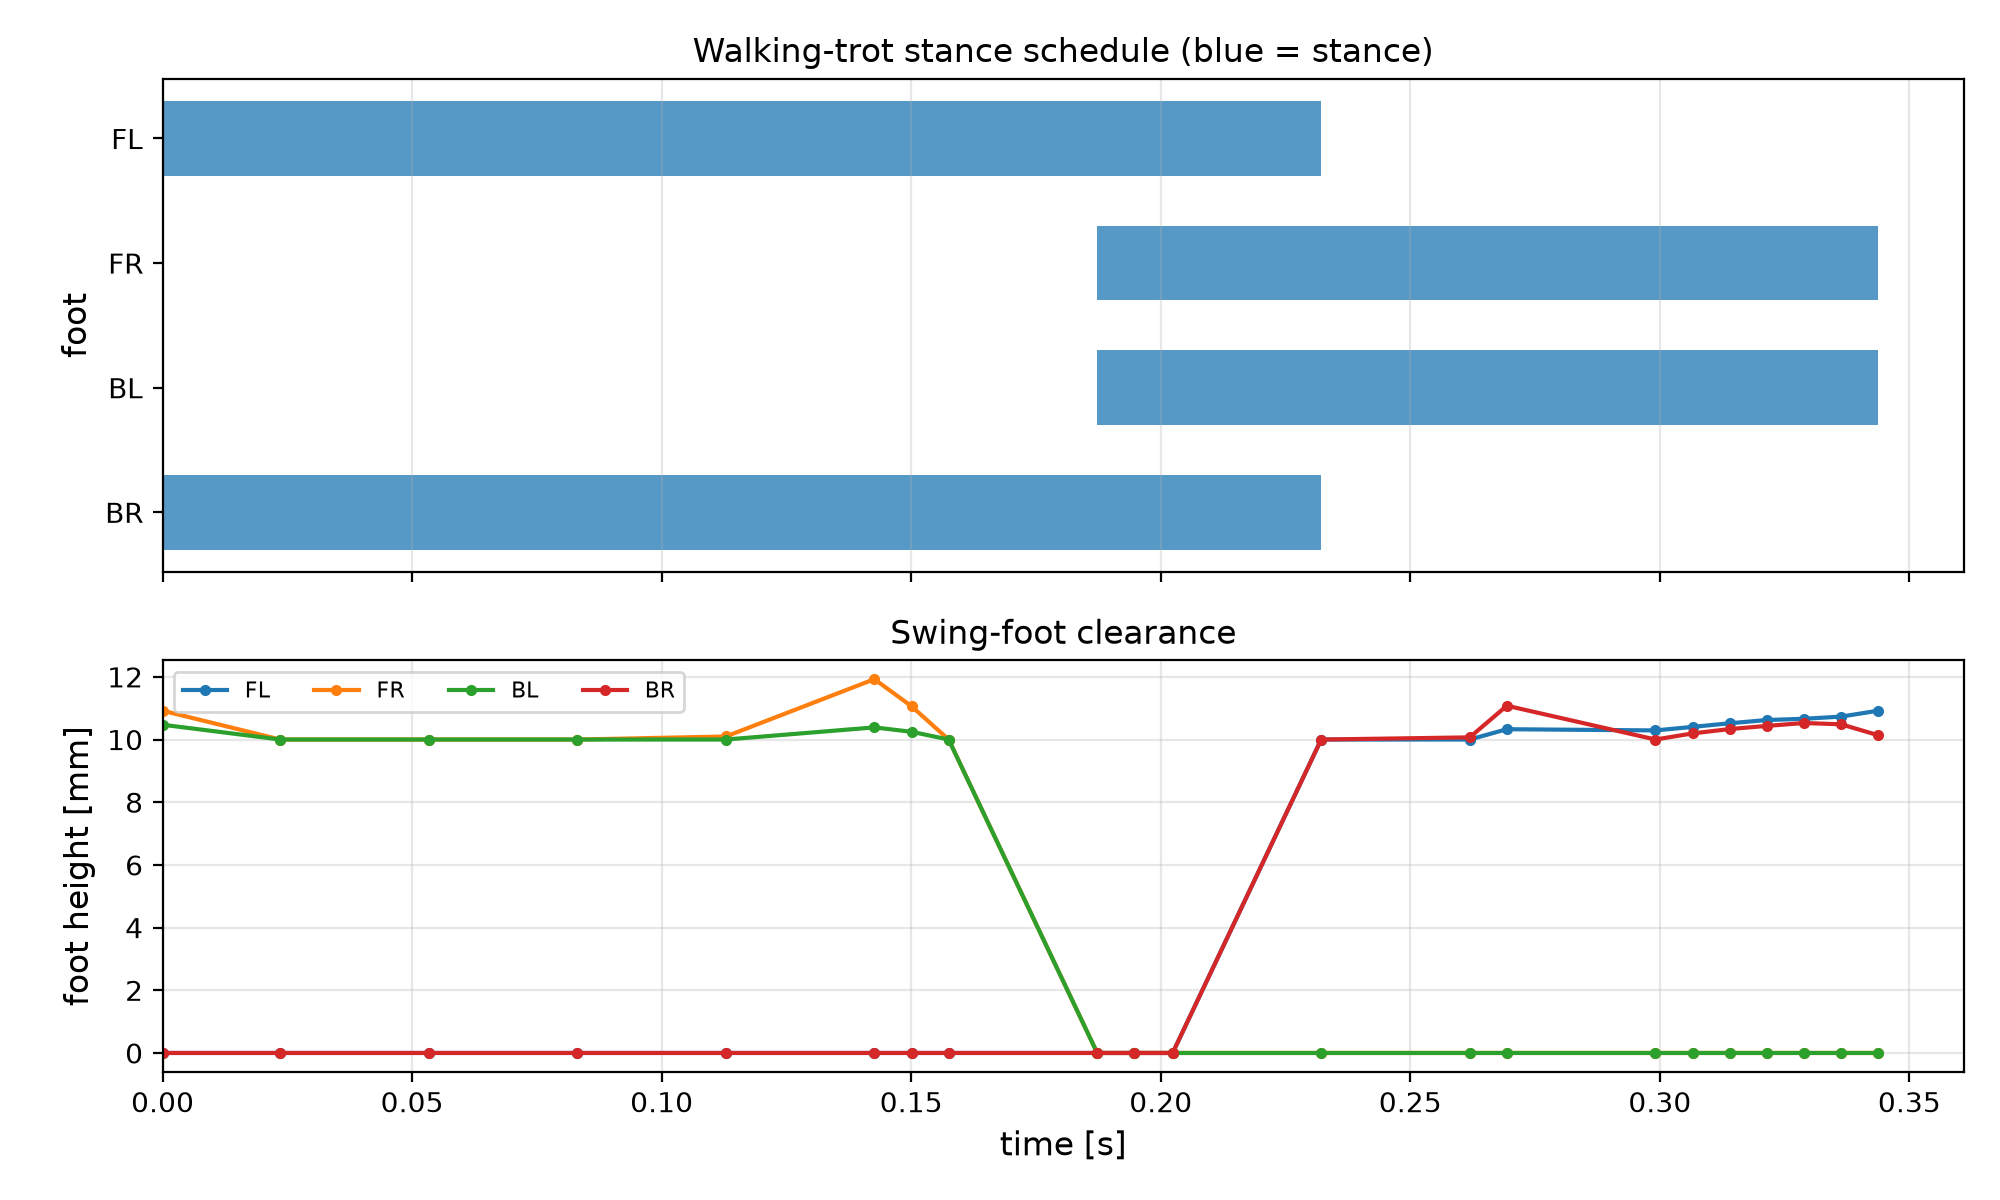
\includegraphics[width=0.95\textwidth]{fig5_8_littledog_gait.png}
  \caption{Example 5.2: walking-trot stance schedule and swing-foot clearance.
  Front-left and back-right are in stance for the first part of the half
  stride, then front-right and back-left take over.  The swing feet clear the
  ground by about 10--12~mm.}
  \label{fig:little_gait}
\end{figure}

\begin{figure}[htbp]
  \centering
  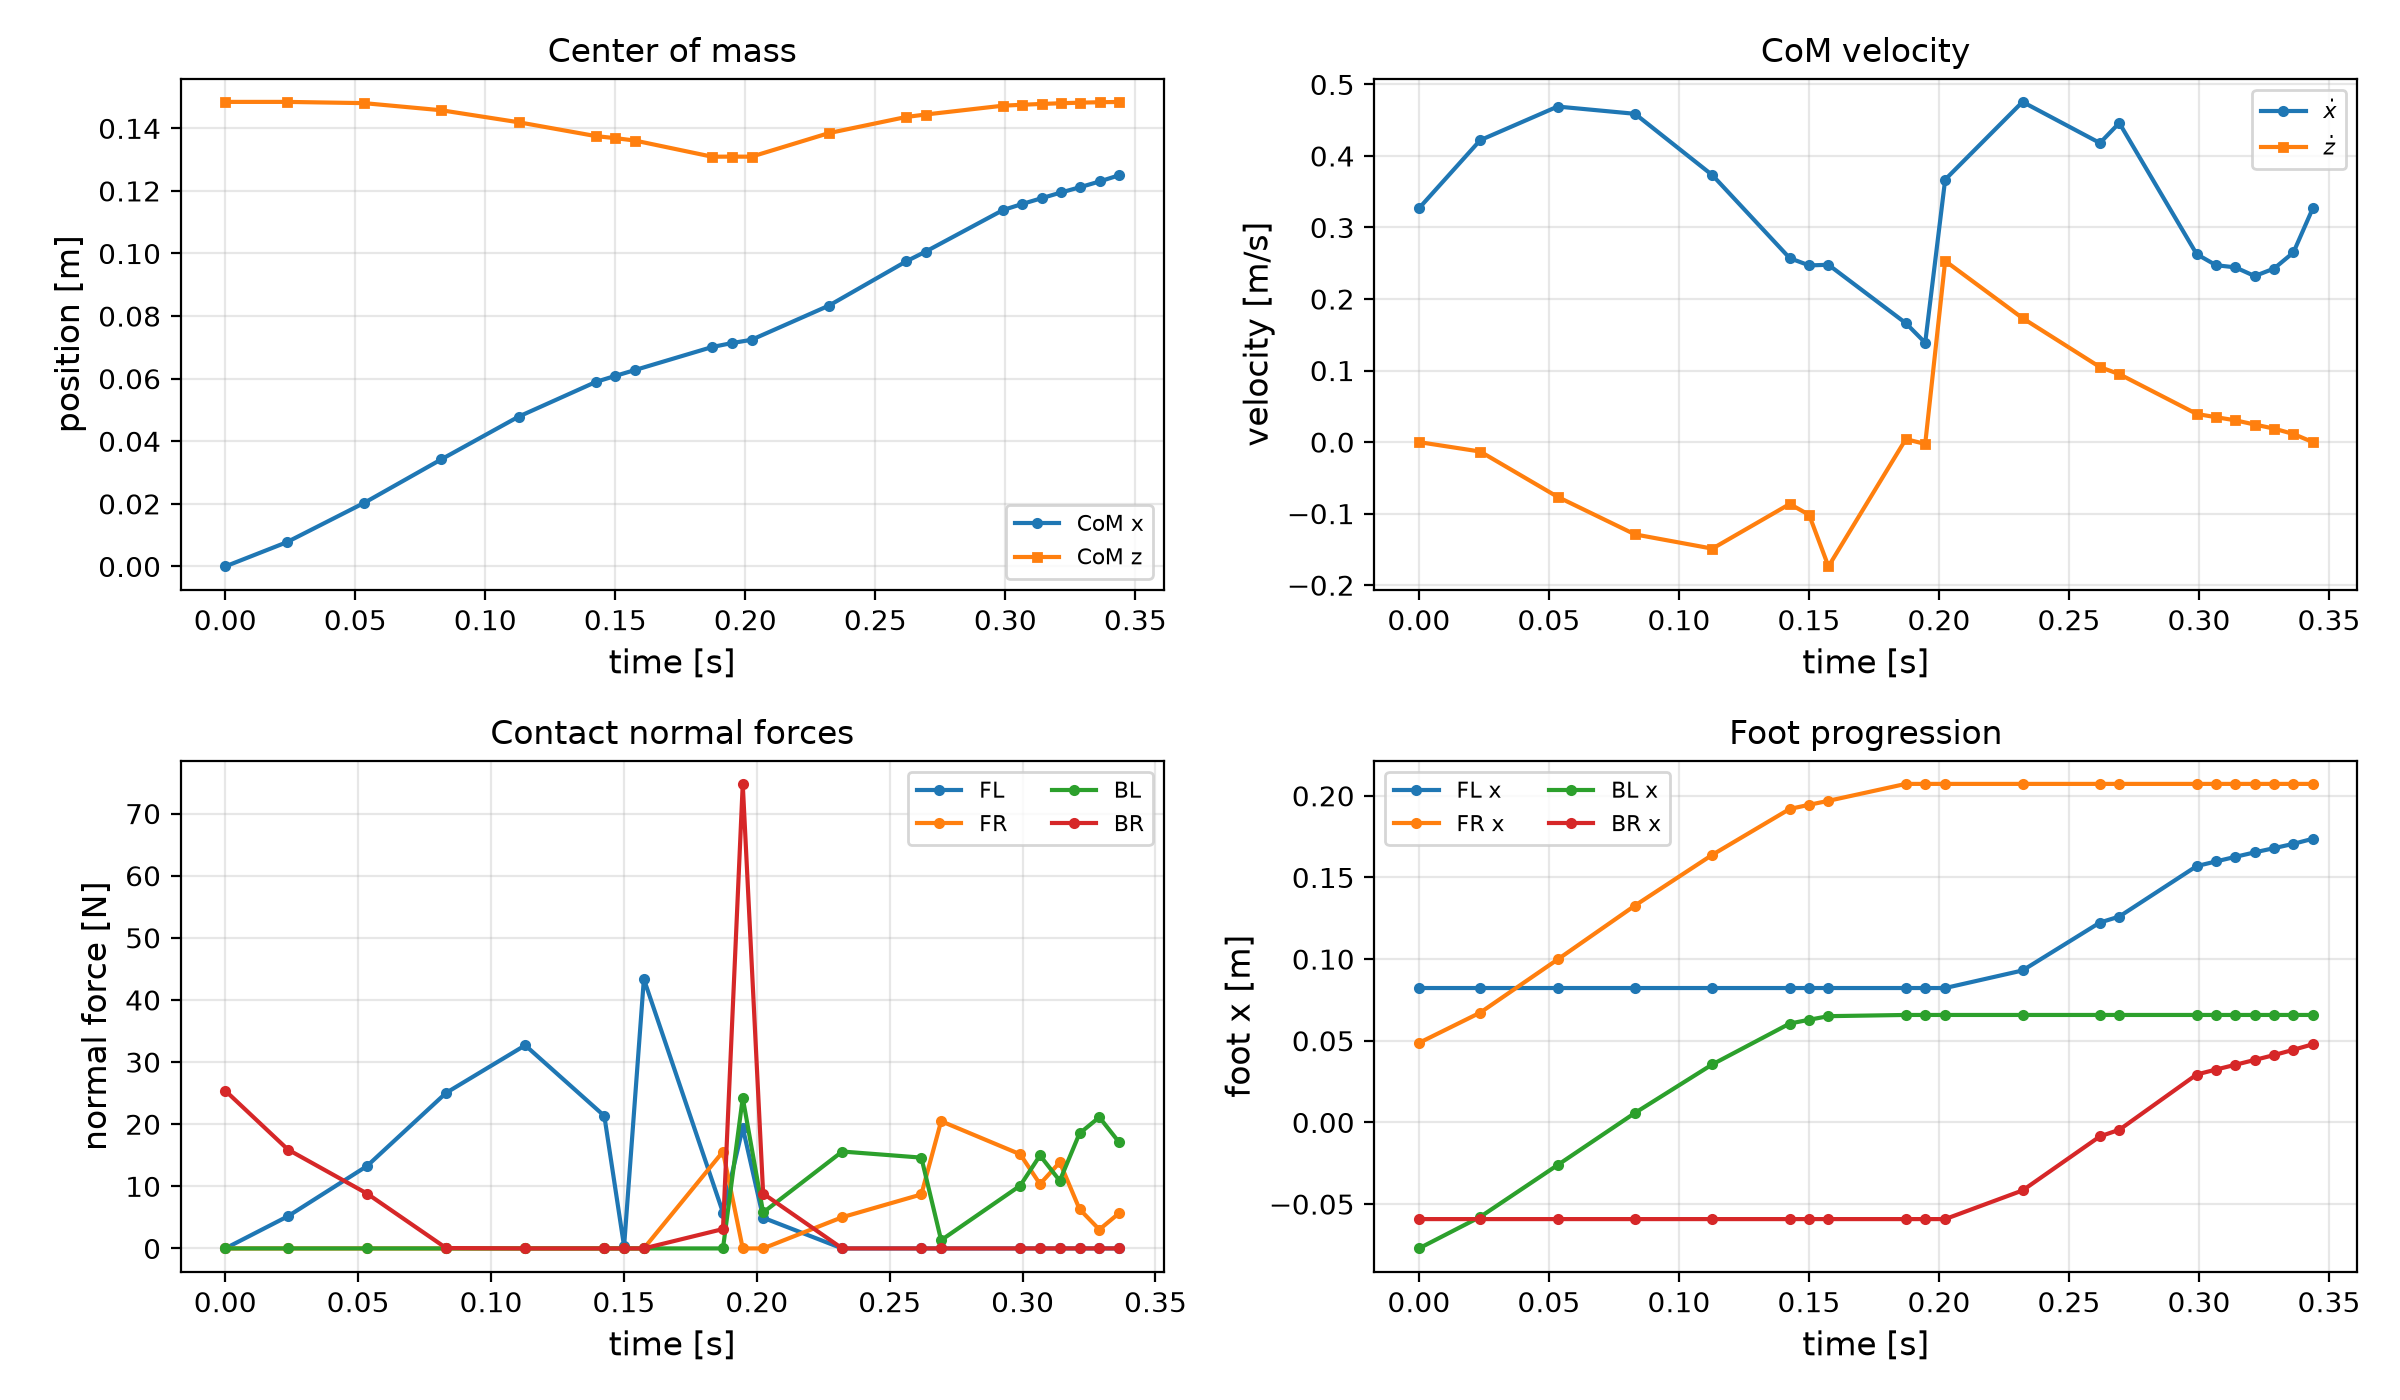
\includegraphics[width=0.98\textwidth]{fig5_9_littledog_state.png}
  \caption{Example 5.2: CoM position and velocity, contact normal forces, and
  foot progression over one half stride.  The normal forces switch between the
  diagonal pairs at the trot transition.}
  \label{fig:little_state}
\end{figure}

\begin{figure}[htbp]
  \centering
  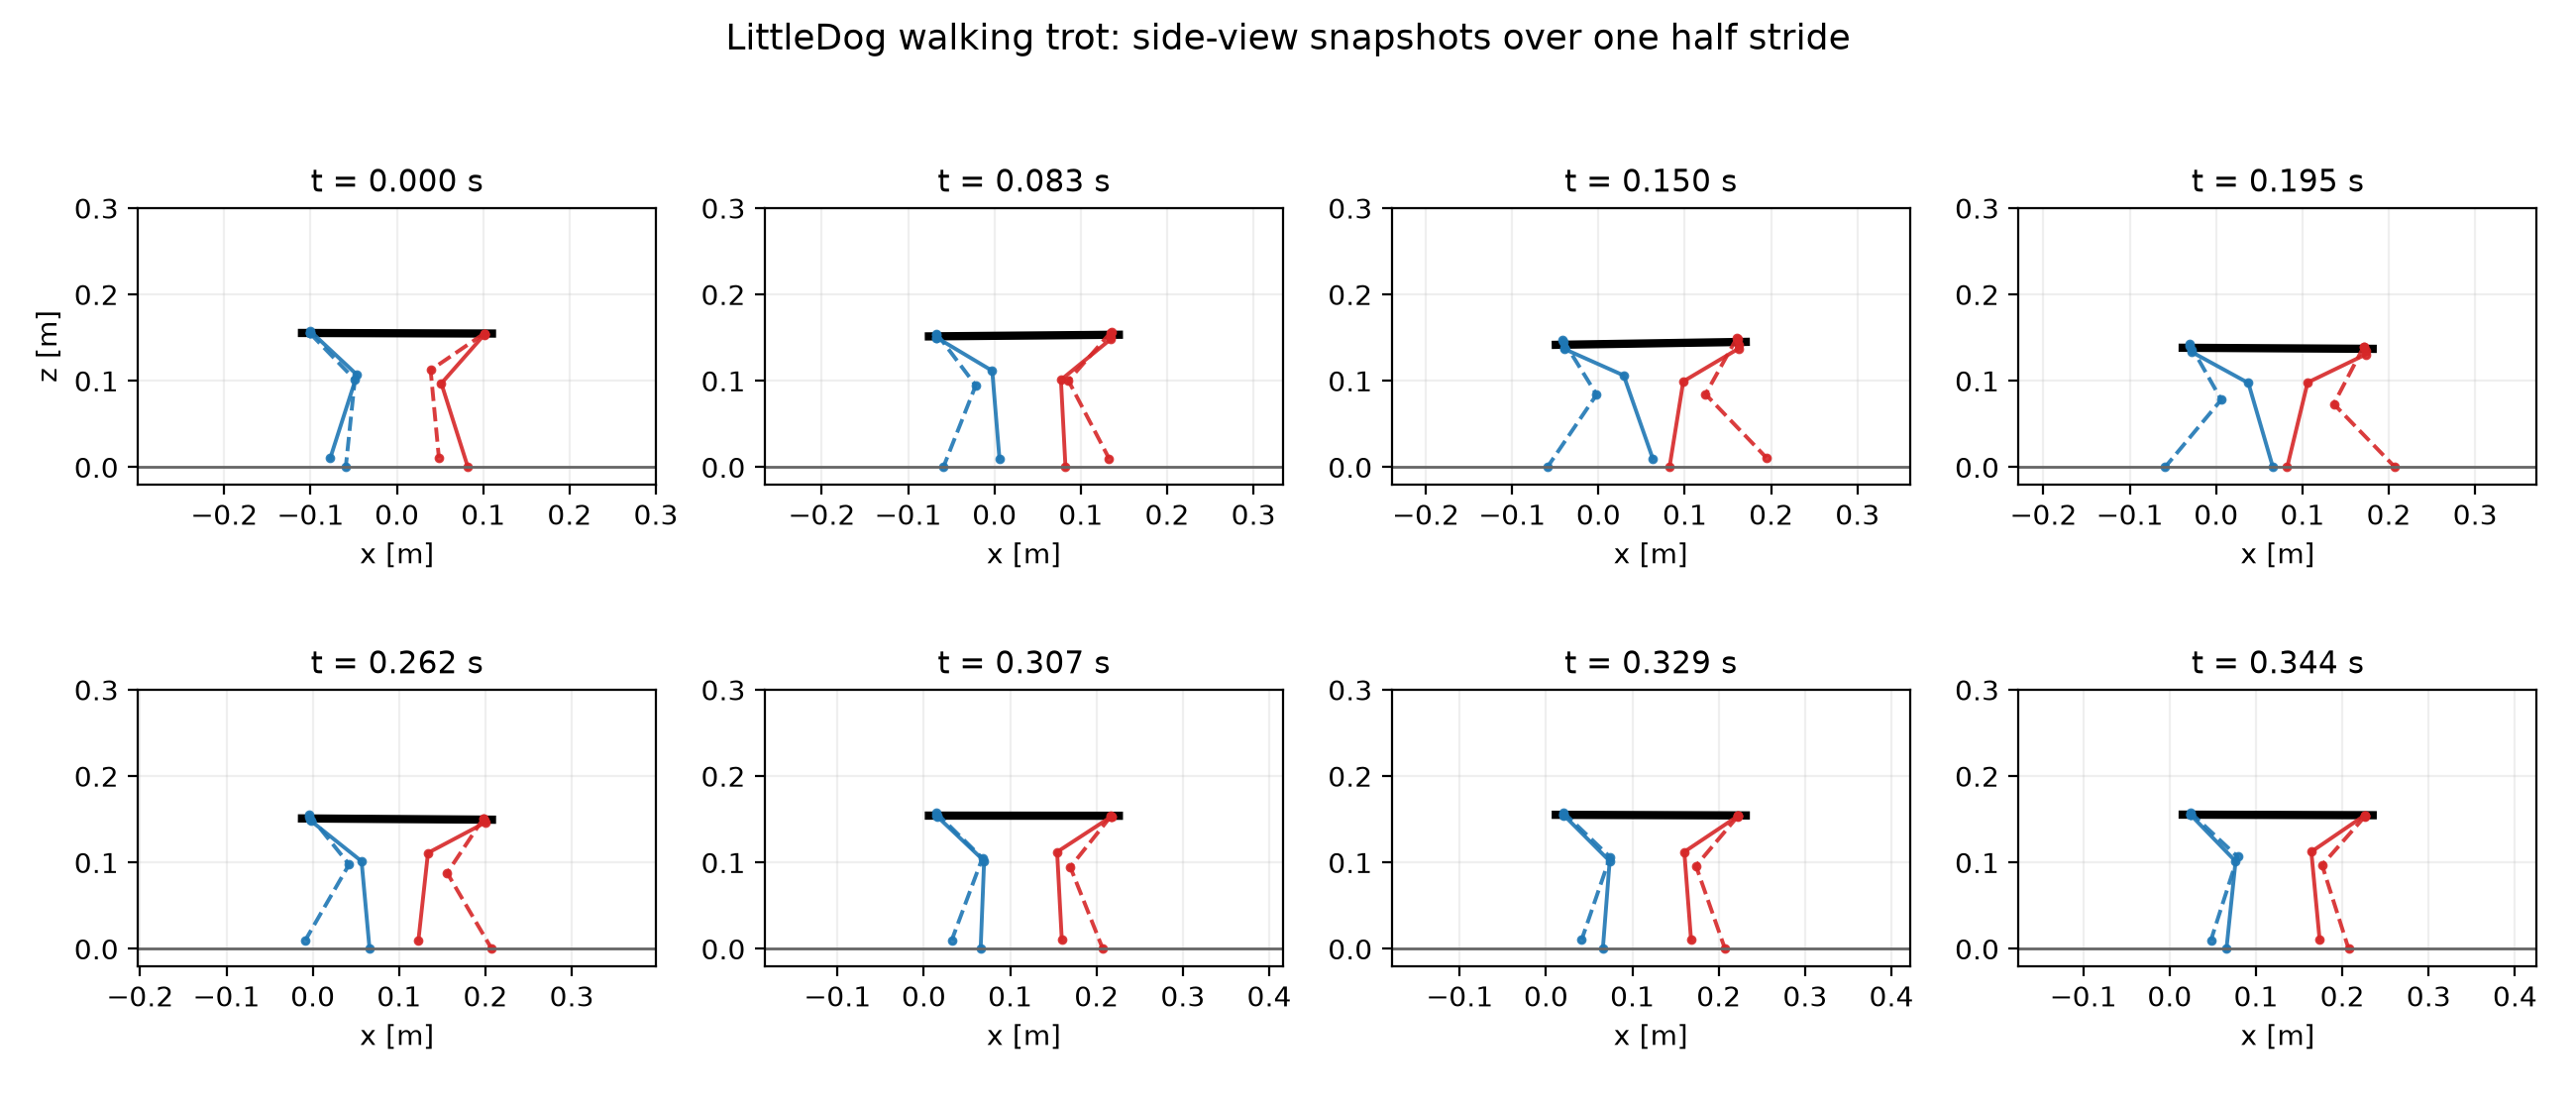
\includegraphics[width=0.98\textwidth]{fig5_10_littledog_snapshots.png}
  \caption{Example 5.2: side-view snapshots of the optimized walking trot over
  one half stride ($t=0$ to $0.344$~s).  Solid legs are left legs, dashed legs
  are right legs; the body is the thick black segment.  The two diagonal pairs
  alternate as expected.}
  \label{fig:little_snapshots}
\end{figure}

\begin{intuition}[breakable=false,title={What the optimizer is actually doing}]
The gait is not prescribed beyond the contact schedule.  The optimizer has to
find joint trajectories whose CoM follows the Newton--Euler equations under
the four contact forces, while each stance foot stays fixed on the ground and
each swing foot clears it.  The angular-momentum constraint couples the
contact forces to the body rotation: if the forces do not pass through the
CoM, the body starts to rotate.  The resulting motion is a compromise between
small joint velocities, small hip-roll motion and the kinematic requirement
that the feet reach the next contact.
\end{intuition}

\textbf{Comments.}  The notebook is explicitly a work in progress: self
collision is not modelled and several costs from the original MATLAB
implementation are missing.  The solution is therefore not necessarily
dynamically feasible in a full simulation; it is a kinematic/centroidal
consistency result.  The value of the example is methodological: it shows how
the exact centroidal dynamics, full kinematics and contact schedules fit into
one nonlinear program, and it shows the role of a good initial guess (the home
configuration) for a local solver.  The walking trot is the easiest of the four
schedules in the notebook; the running trot, rotary gallop and bound are more
aggressive and are left commented out.

\begin{pitfall}[breakable=false,title={A feasible NLP solution is not a stable gait}]
The optimization produces an open-loop trajectory over one half stride.  Nothing
in the program guarantees that the gait is stable to perturbations.  Orbital
stability would require a step-to-step (Poincar\'e) analysis, as in
Chapter~4, or a feedback controller that tracks the trajectory.  The periodic
boundary conditions only make the trajectory repeat, not converge.
\end{pitfall}

%=====================================================================
\section{Section 5.8(a): Footstep Planning via MIQP}
%=====================================================================

\subsection{Terrain and decision variables}

The terrain consists of rectangular stepping stones: an initial stone, a goal
stone, a lateral stone above the bridge, and a sequence of bridge stones with
a boolean presence mask.  Terrain~A has all four bridge stones
(\texttt{[1,1,1,1]}); terrain~B misses the last one (\texttt{[1,1,1,0]}).

The planner uses $n_{\rm steps}+1$ footsteps.  The decision variables are
\begin{itemize}[leftmargin=1.5em]
  \item $\bp^{L}_t,\bp^{R}_t\in\mathbb{R}^2$ for $t=0,\dots,n_{\rm steps}$;
  \item binaries $\delta^{L}_{t,i},\delta^{R}_{t,i}\in\{0,1\}$, one per foot,
        step and stone;
  \item a binary \texttt{first\_left} that decides which foot moves first.
\end{itemize}

\subsection{The four constraints and the objective}

The four pieces requested by the exercise are the following.

\paragraph{(a) Relative position limit.}  At every step each foot must lie in a
square of side $d$ centered at the other foot:
\begin{equation}
\left|\bp^{L}_t-\bp^{R}_t\right|_\infty\le \frac{d}{2},
\qquad t=0,\dots,n_{\rm steps}.
\label{eq:rel_limit}
\end{equation}

\paragraph{(b) One stone per foot.}  A foot cannot be in two stones at once:
\begin{equation}
\sum_i \delta^{L}_{t,i}=1,\qquad
\sum_i \delta^{R}_{t,i}=1 .
\label{eq:one_stone}
\end{equation}

\paragraph{(c) Foot in the assigned stone (big-M).}  With the halfspace
representation $S_i=\{x:A_ix\le b_i\}$,
\begin{equation}
A_i\bp^{L}_t\le b_i+(1-\delta^{L}_{t,i})M,\qquad
A_i\bp^{R}_t\le b_i+(1-\delta^{R}_{t,i})M,
\label{eq:bigm}
\end{equation}
where $M$ is a vector of two ``sufficiently large'' positive constants (one
per coordinate), chosen from the terrain extents.  If $\delta_{t,i}=1$ the
constraint enforces membership in stone $i$; otherwise it is relaxed.  The
other binary at that step is zero by~\eqref{eq:one_stone}, so the foot cannot
be simultaneously required to be in two stones.

\paragraph{(d) Step-length objective.}  Minimize the sum of squared step
lengths,
\begin{equation}
\min\;\sum_{t=0}^{n_{\rm steps}-1}
\left(
\|\bp^{L}_{t+1}-\bp^{L}_t\|^2
+\|\bp^{R}_{t+1}-\bp^{R}_t\|^2
\right).
\label{eq:miqp_cost}
\end{equation}
The step-sequence constraint (given in the notebook) uses the binary
\texttt{first\_left} to allow only one foot to move per step, alternating feet;
it is a big-M constraint with $M=d$ on the square centered at the previous
position of the same foot.

The resulting MIQP is solved with Drake's \texttt{MixedIntegerBranchAndBound},
using OSQP for the continuous relaxations.

\subsection{Results on the two benchmark terrains}

\begin{figure}[htbp]
  \centering
  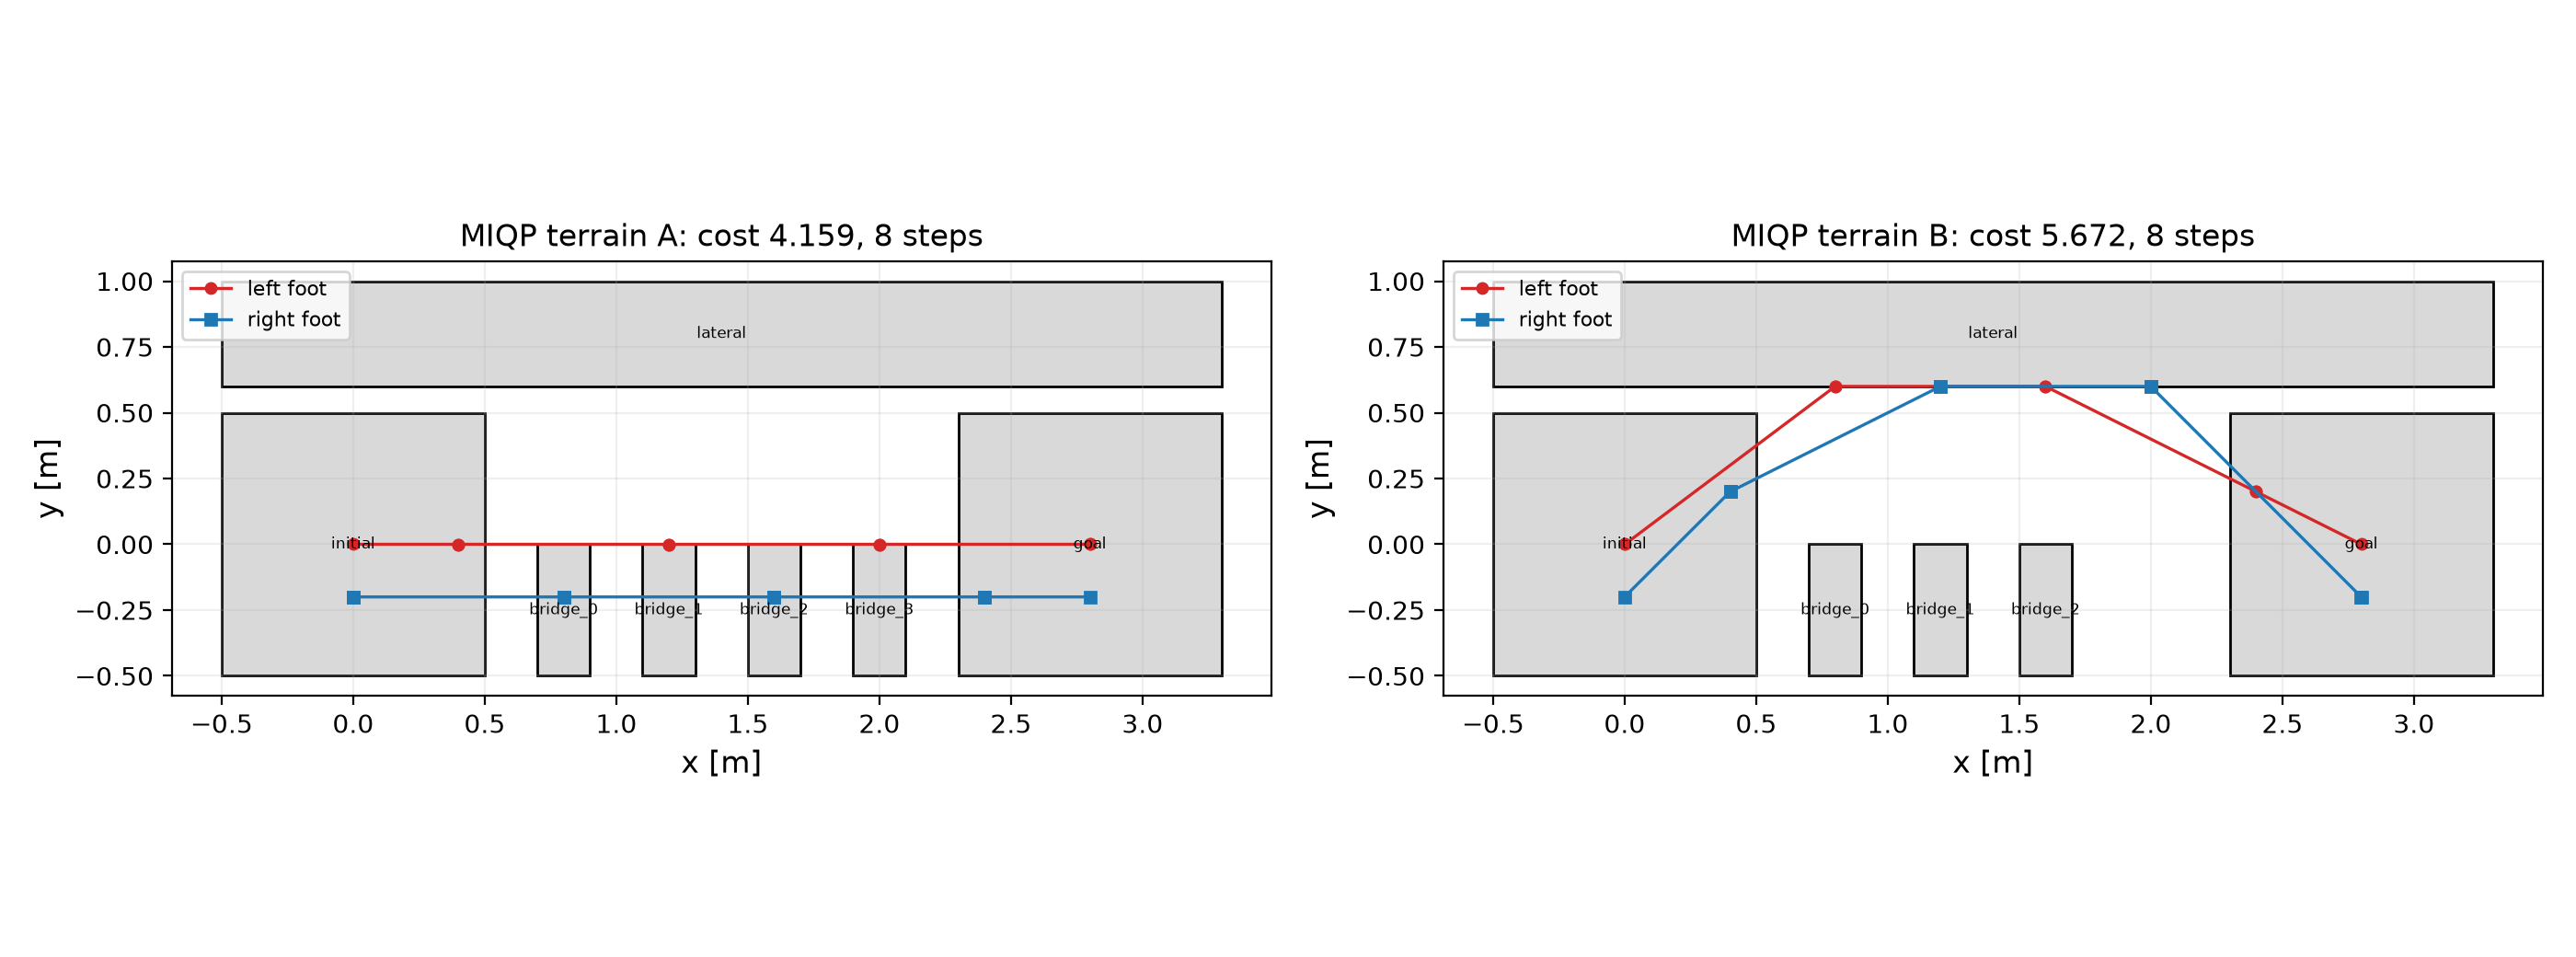
\includegraphics[width=0.98\textwidth]{fig5_4_miqp_plans.png}
  \caption{Section 5.8(a): optimal MIQP plans.  Terrain~A goes straight across
  the bridge; terrain~B must use the lateral stone because the missing bridge
  stone leaves a gap that is too wide under the step-span and foot-separation
  limits.}
  \label{fig:miqp_plans}
\end{figure}

\begin{table}[H]
\centering
\caption{Section 5.8(a): MIQP results ($n_{\rm steps}=8$, $d=0.8$~m).}
\begin{tabular}{cccccc}
\toprule
Terrain & cost & solve time [s] & steps used & route & first foot \\
\midrule
A \texttt{[1,1,1,1]} & 4.1593 & 0.42 & 8 & bridge & left \\
B \texttt{[1,1,1,0]} & 5.6721 & 0.75 & 8 & lateral & right \\
\bottomrule
\end{tabular}
\end{table}

The autograder reports
\begin{center}
\textbf{Total score is 16/16: relative position 4/4, one stone per foot 3/3,
foot in stone 5/5, objective 4/4.}
\end{center}
The objective value for terrain~A agrees with the reference value
$4.1592510194$ to $10^{-10}$; for terrain~B the value $5.6721$ is within the
autograder's 2\% tolerance of $5.6479$.  The small difference comes from the
branch-and-bound convergence tolerance, not from a modelling error.

\begin{intuition}[breakable=false,title={Why the lateral stone is used in terrain B}]
The last bridge stone is missing.  The remaining bridge ends at $x=1.7$~m,
while the goal stone starts at $x=2.3$~m: a 0.6~m gap.  With $d=0.8$~m the
feet may be at most $0.4$~m apart, so a foot on the last bridge stone cannot
reach the goal.  The lateral stone is high enough and long enough to provide
intermediate footholds; the optimizer chooses it even though the path is
longer.  This is exactly the kind of non-local decision that a local
continuous optimizer would miss and branch and bound handles naturally.
\end{intuition}

\subsection{Step-span sensitivity and route switching}

We swept $d$ from 0.6 to 1.5~m on terrain~B (all other parameters fixed).

\begin{table}[H]
\centering
\caption{Section 5.8(a): step-span sensitivity on terrain~B.}
\begin{tabular}{cccl}
\toprule
$d$ [m] & cost & steps used & route \\
\midrule
0.60 & -- & -- & infeasible \\
0.70 & -- & -- & infeasible \\
0.75 & -- & -- & infeasible \\
0.80 & 5.6721 & 8 & lateral \\
0.90 & 5.5916 & 8 & lateral \\
1.00 & 5.4091 & 8 & lateral \\
1.10 & 5.3740 & 8 & lateral \\
1.20 & 4.1873 & 8 & bridge \\
1.30 & 4.1655 & 8 & bridge \\
1.40 & 4.0317 & 8 & bridge \\
1.50 & 4.0252 & 8 & bridge \\
\bottomrule
\end{tabular}
\end{table}

\begin{figure}[htbp]
  \centering
  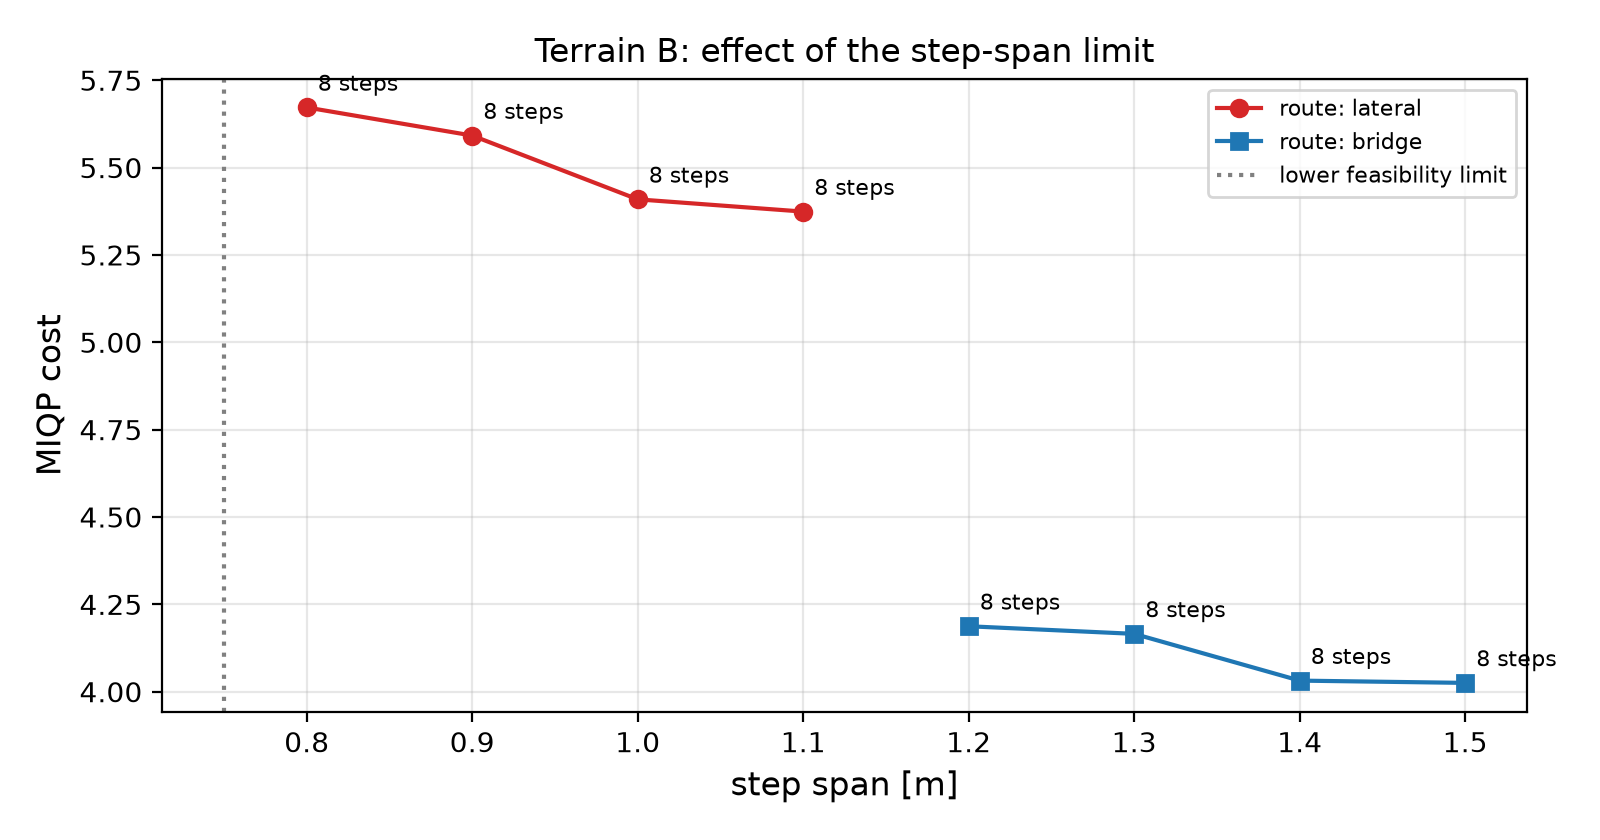
\includegraphics[width=0.75\textwidth]{fig5_6_span_sensitivity.png}
  \caption{Section 5.8(a): cost versus step span on terrain~B.  The route
  switches from the lateral stone to the bridge between $d=1.1$ and
  $d=1.2$~m.}
  \label{fig:span_sensitivity}
\end{figure}

There are two thresholds.  Below $d=0.8$~m the problem is infeasible: the feet
cannot be placed on the narrow (0.2~m wide) bridge stones while remaining
within $d/2$ of each other and making progress.  Between $0.8$ and $1.1$~m the
lateral route is feasible but the bridge is not.  At $d=1.2$~m the feet may be
$0.6$~m apart, which is exactly the gap from the last bridge stone to the goal;
the planner switches to the shorter bridge route and the cost drops from
$5.37$ to $4.19$.  Above $1.2$~m the bridge route remains optimal and the cost
decreases slowly as the squared step lengths shrink.

\textbf{Comments.}  The MIQP is a clean example of a combinatorial problem with
continuous geometry.  The binaries encode the discrete choice ``which stone''
and the big-M constraints encode the implication ``if this binary is one, the
foot is in this rectangle''.  The objective is convex quadratic, so branch and
bound is guaranteed to find the global optimum.  The price is exponential
worst-case complexity in the number of binaries, which is why the exercise
uses only four bridge stones and eight steps.

%=====================================================================
\section{Section 5.8(b): Understanding the Zero-Moment Point}
%=====================================================================

\subsection{Free-body diagrams}

We use the geometry of Fig.~\ref{fig:foot_geometry}: the heel is $H$, the toe
is $T$, the ankle pin is $P$ at height $h$, the ankle is $L_2$ from the heel
and $L_1$ from the toe, and the leg of length $l$ carries a point mass $m$.
The angle $\theta$ is measured from the horizontal at $P$.

\begin{figure}[htbp]
  \centering
  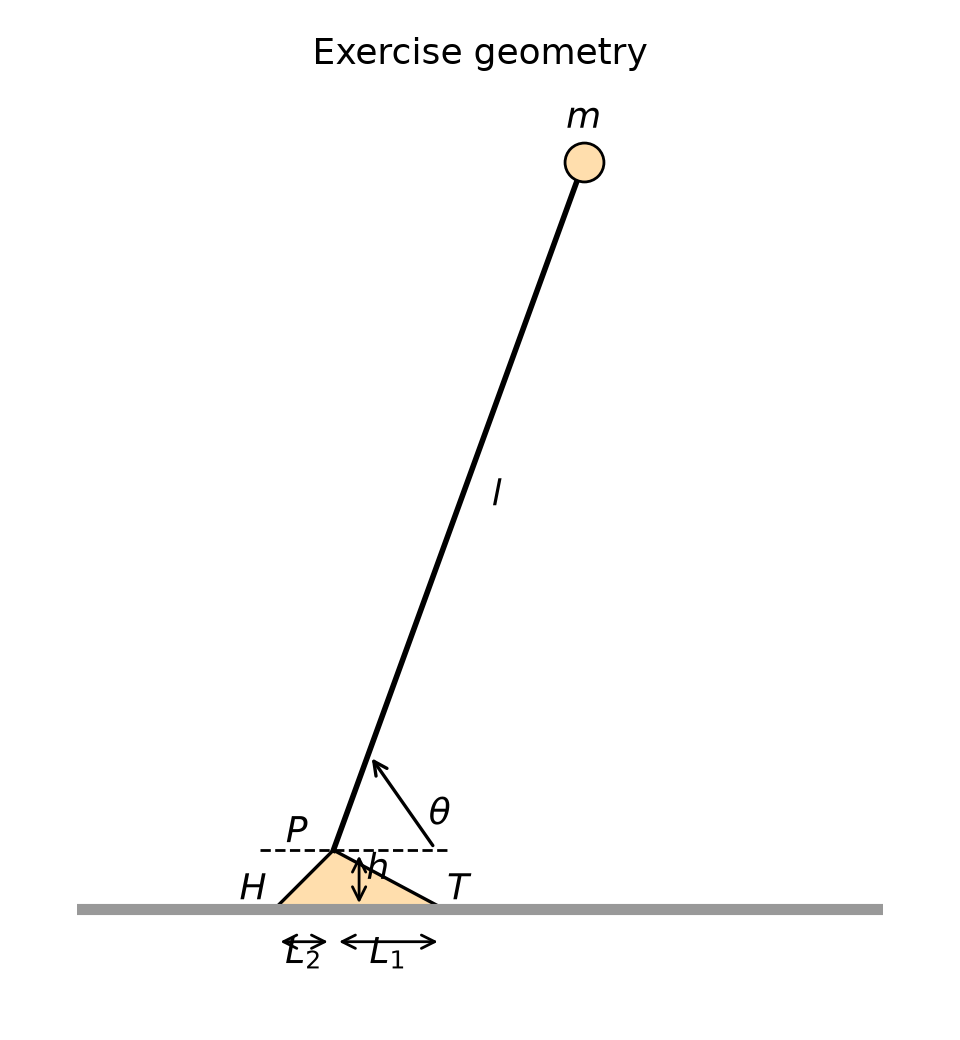
\includegraphics[width=0.42\textwidth]{fig5_12_foot_geometry.png}
  \caption{Geometry of the Section 5.8(b) exercise.  The foot is the triangle
  $HPT$; the massless leg $l$ carries the point mass $m$; $\theta$ is measured
  from the horizontal at the ankle $P$.}
  \label{fig:foot_geometry}
\end{figure}

\paragraph{(a) Free-body diagrams.}
\begin{itemize}[leftmargin=1.5em]
  \item \emph{Bob:} gravity $m\mathbf{g}$ downward and the leg force along the
        leg (the leg can only push or pull along its axis).
  \item \emph{Leg:} massless; the forces at the two pins are equal and
        opposite along the leg.  It is a two-force member.  There is no torque
        at either pin.
  \item \emph{Foot:} the force from the leg at $P$, the ground reactions at
        $H$ and $T$ (normal and friction), and no ankle torque for parts
        (a)--(d).  Because the foot is massless, the sum of forces and the sum
        of moments about any point vanish.
\end{itemize}

\paragraph{(b) Stability at $\theta=\pi/2+10^{-3}$.}
The leg is a pendulum about $P$:
\begin{equation}
\ddot{\theta}=-\frac{g}{l}\cos\theta .
\end{equation}
At $\theta=\pi/2+\varepsilon$ we have $\cos\theta=-\sin\varepsilon\approx
-\varepsilon$, so
\begin{equation}
\ddot{\theta}\approx\frac{g}{l}\varepsilon>0 .
\end{equation}
The perturbation grows exponentially with rate $\sqrt{g/l}$ (about
$3.13$~s$^{-1}$ for $l=1$~m): the posture is \emph{unstable}.  The ZMP is at
$x_{\rm ZMP}=-h\cot\theta\approx h\varepsilon$ (toward the toe), which is
inside the foot for small $\varepsilon$; the \emph{foot} stays flat while the
\emph{body} falls.  This distinction is important: foot-flatness and postural
stability are different properties.

\subsection{(c) The ZMP without an ankle actuator}

Because the leg is a two-force member, the force it exerts on the foot at $P$
is along the line $P$--bob.  The ground reaction must balance this force, so
the resultant ground reaction is also along that line.  The ZMP is therefore
the intersection of the line $P$--bob with the ground.  Taking $P$ as the
origin,
\[
P=(0,h),\qquad \text{bob}=(l\cos\theta,\,h+l\sin\theta).
\]
The line through these points hits $z=0$ at
\begin{equation}
\boxed{x_{\rm ZMP}(\theta)=-h\cot\theta .}
\label{eq:zmp_free}
\end{equation}
The result is independent of $\dot\theta$ and of $m$: it is a purely geometric
statement about the line of action.  The equivalent derivation from the general
ZMP formula
\[
x_{\rm ZMP}=x_{\rm cm}-\frac{z_{\rm cm}\,\ddot{x}_{\rm cm}}
{\ddot{z}_{\rm cm}+g}
\]
uses $\ddot{x}_{\rm cm}=g\sin\theta\cos\theta-l\cos\theta\,\dot\theta^2$ and
$\ddot{z}_{\rm cm}=-g\cos^2\theta-l\sin\theta\,\dot\theta^2$; the
$\dot\theta$ terms cancel and give the same
expression~\eqref{eq:zmp_free}.

\paragraph{(d) Toe and heel boundaries.}
With the foot support $[-L_2,L_1]$ relative to $P$:
\begin{align}
x_{\rm ZMP}=L_1 &\;\Longrightarrow\;
\theta_T=\pi-\arctan\frac{h}{L_1},
\label{eq:theta_T}\\
x_{\rm ZMP}=-L_2 &\;\Longrightarrow\;
\theta_H=\arctan\frac{h}{L_2}.
\label{eq:theta_H}
\end{align}
At $\theta_T$ the ZMP reaches the toe.  Beyond it the resultant would lie ahead
of the toe, so the foot rotates about $T$ and the \emph{heel lifts}.  At
$\theta_H$ the ZMP reaches the heel; the foot rotates about $H$ and the
\emph{toe lifts}.  For the numerical values in
Fig.~\ref{fig:zmp_exercise} ($h=0.08$~m, $L_1=0.15$~m, $L_2=0.08$~m) we get
\[
\theta_T=151.9^\circ,\qquad \theta_H=45.0^\circ .
\]
The counter-intuitive sign is worth emphasizing: because the leg is a strut
with a frictionless ankle, leaning \emph{backward} pushes the ZMP
\emph{forward} toward the toe, and leaning forward pushes it toward the heel.

\subsection{(e)--(f) With an ideal ankle actuator}

Now the ankle applies a torque that exactly cancels the gravitational torque
on the leg, so $\ddot\theta=0$.  The robot is quasi-static and the ankle torque
is internal to the robot.  The only external forces are gravity at the CoM and
the ground reaction; for zero moment about the CoM the ground reaction must
pass through the CoM.  Hence the ZMP is the vertical projection of the CoM:
\begin{equation}
\boxed{x_{\rm ZMP}(\theta)=l\cos\theta .}
\label{eq:zmp_actuated}
\end{equation}
The flat-foot condition $x_{\rm ZMP}\in[-L_2,L_1]$ gives
\begin{equation}
\theta\in\left[
\arccos\!\left(\frac{L_1}{l}\right),\;
\arccos\!\left(-\frac{L_2}{l}\right)
\right],
\label{eq:theta_range}
\end{equation}
with the arguments clipped to $[-1,1]$.  For the numerical values above this
is $[81.4^\circ,94.6^\circ]$, a range of only $13.2^\circ$.

\paragraph{(e) About to fall.}
If the robot is about to tip forward, the heel normal force is zero and the
ZMP is at the toe; if it is about to tip backward, the toe normal force is zero
and the ZMP is at the heel.  In either case one of the two ground reaction
forces vanishes and the ZMP is on the boundary of the support polygon.

\subsection{(g)--(h) Foot design}

\paragraph{(g) Maximizing the posture range.}
\begin{enumerate}[label=(\roman*),leftmargin=1.8em]
  \item \emph{Taller or flatter?}  In the static
        expression~\eqref{eq:zmp_actuated}, $h$ does not appear: the achievable
        range~\eqref{eq:theta_range} depends only on $L_1,L_2,l$.  A taller foot
        does not change the static range.  Dynamically, however, horizontal
        ground forces produce a moment $hF_x$ about the ankle; a flatter foot
        (smaller $h$) reduces the ankle torque needed for a given horizontal
        force, so a flatter foot is preferable in practice.
  \item \emph{Longer or shorter?}  A longer foot (larger $L_1+L_2$) enlarges
        the support polygon and therefore the range.  For $L_1=L_2=0.115$~m
        and $l=1$~m the range is $13.2^\circ$; for $L_1=L_2=0.20$~m it is
        $23.1^\circ$.
  \item \emph{Where to put the ankle?}  For a fixed total length $L=L_1+L_2$,
        the range~\eqref{eq:theta_range} is almost independent of the ankle
        placement: centering gives $13.21^\circ$ for $L=0.23$~m, while putting
        the ankle at one end gives $13.28^\circ$, a difference of
        $0.07^\circ$.  The total length is what matters.  If a slight bias is
        wanted, placing the ankle at one end maximizes the total range, while
        centering maximizes the minimum margin on both sides.  For symmetric
        posture robustness, center the ankle.
\end{enumerate}

\paragraph{(h) Designing for forward walking and easy heel lift.}
\begin{enumerate}[label=(\roman*),leftmargin=1.8em]
  \item \emph{Taller or flatter?}  The quasi-static heel-lift condition is
        $l\cos\theta=L_1$, which is independent of $h$; statically, $h$ does
        not matter.  Dynamically, a flatter foot reduces the ankle torque
        associated with horizontal push-off forces, so flatter is again
        preferable.
  \item \emph{Longer or shorter $L_1$?}  A shorter $L_1$ moves the toe closer
        to the CoM projection and makes heel lift occur at a more upright
        posture.  The ankle torque needed to reach the toe,
        $mg(L_1-l\cos\theta)$, also decreases with $L_1$.  So a \emph{shorter}
        forefoot makes heel lift easier.
  \item \emph{Longer or shorter $L_2$?}  $L_2$ does not enter the heel-lift
        condition; it sets the \emph{backward} support margin and prevents toe
        lift.  A longer heel does not make heel lift easier, but it improves
        backward stability during stance.  For forward walking the useful
        design is a short $L_1$ (easy heel lift) combined with a sufficiently
        long $L_2$ (backward safety).
\end{enumerate}

\begin{figure}[htbp]
  \centering
  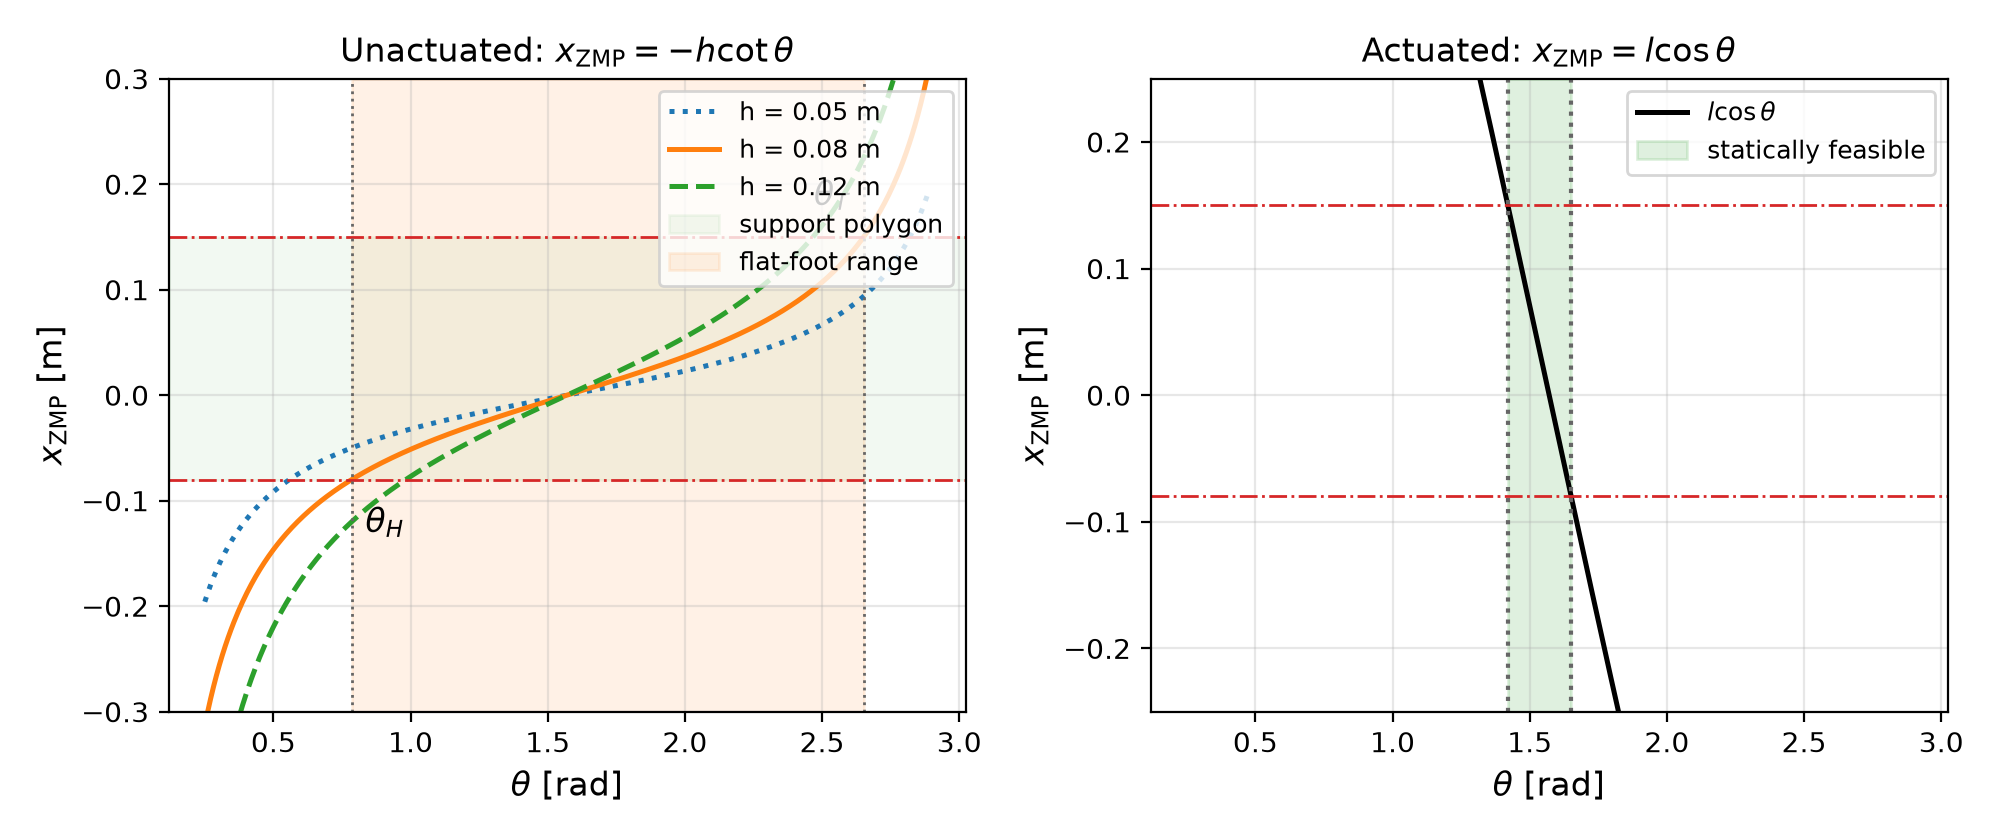
\includegraphics[width=0.98\textwidth]{fig5_11_zmp_exercise.png}
  \caption{Section 5.8(b).  Left: unactuated case,
  $x_{\rm ZMP}=-h\cot\theta$ for three ankle heights; the shaded horizontal
  band is the support polygon and the vertical band is the flat-foot range.
  Right: with an ideal ankle actuator the ZMP is $l\cos\theta$; the
  statically feasible interval is narrow for a short foot.}
  \label{fig:zmp_exercise}
\end{figure}

\begin{pitfall}[breakable=false,title={Heel lift is not ``the ZMP reaches the heel''}]
The heel lifts when the ground reaction resultant reaches the \emph{toe}: the
heel normal force becomes zero there.  When the resultant reaches the
\emph{heel}, the \emph{toe} lifts.  It is easy to say this backwards.  The
rule is: the foot rotates about the edge that the ZMP is approaching, and the
opposite edge leaves the ground.
\end{pitfall}

%=====================================================================
\section{Section 5.8(c): Footstep Planning via GCS}
%=====================================================================

\subsection{Transcription}

The GCS formulation removes the binaries.  Each stepping stone is a convex
set, and each possible visit is a \emph{copy} of that set, i.e.\ a vertex of
the graph.  A stone of horizontal length $L$ gets
\begin{equation}
m=\left\lfloor \frac{L}{d}\right\rfloor+2
\end{equation}
copies: enough variables to cross the stone in several steps and to place both
feet on it.  The source and target are singleton sets at the centers of the
initial and goal stones.

The edges are:
\begin{itemize}[leftmargin=1.5em]
  \item consecutive copies of the same stone: $x_{i,0}\to x_{i,1}\to\cdots$;
  \item from a copy of one stone to the \emph{parent} copy ($ii=0$) of another
        stone;
  \item from any copy of the goal stone to the target;
  \item from the source to the parent copy of any stone.
\end{itemize}
Each edge carries the kinematic constraint
\begin{equation}
\|x_u-x_v\|_\infty\le \frac{d}{2},
\end{equation}
which is the same foot-separation limit as~\eqref{eq:rel_limit}, and a constant
cost of 1 (one step).  The planner then solves a shortest-path problem in the
graph, with the convex relaxation of the bilinear flow constraints.  The
relaxation is tight for this problem: the flow variables take values 0 or 1 in
the solution, and Drake's rounding step is not needed to recover the path.

\begin{figure}[htbp]
\centering
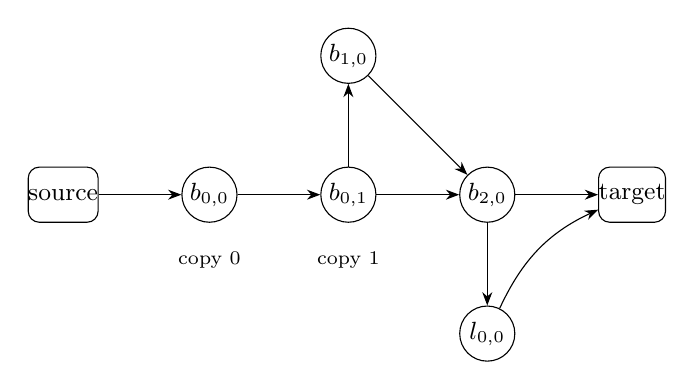
\begin{tikzpicture}[>=Stealth,node distance=1.05cm,scale=1.0,
  every node/.style={font=\small},
  v/.style={circle,draw,minimum size=7mm,inner sep=0pt},
  s/.style={rectangle,draw,rounded corners,minimum size=7mm,inner sep=0pt}]
  \node[s] (src) {source};
  \node[v,right=of src] (b0) {$b_{0,0}$};
  \node[v,right=of b0] (b1) {$b_{0,1}$};
  \node[v,above=of b1] (b2) {$b_{1,0}$};
  \node[v,right=of b1] (b3) {$b_{2,0}$};
  \node[v,below=of b3] (l0) {$l_{0,0}$};
  \node[s,right=of b3] (tgt) {target};
  \draw[->] (src)--(b0);
  \draw[->] (b0)--(b1);
  \draw[->] (b1)--(b2);
  \draw[->] (b1)--(b3);
  \draw[->] (b2)--(b3);
  \draw[->] (b3)--(tgt);
  \draw[->] (b3)--(l0);
  \draw[->] (l0) to[bend left=20] (tgt);
  \node[font=\scriptsize,below=0.25cm of b0] {copy 0};
  \node[font=\scriptsize,below=0.25cm of b1] {copy 1};
\end{tikzpicture}
\caption{Schematic of the GCS for Section 5.8(c).  Vertices are copies of
stepping stones; edges are feasible one-step transitions.  A path from
\texttt{source} to \texttt{target} is a footstep plan.  The copies of the same
stone are chained in a fixed order.}
\label{fig:gcs_graph}
\end{figure}

\subsection{Results}

\begin{figure}[htbp]
  \centering
  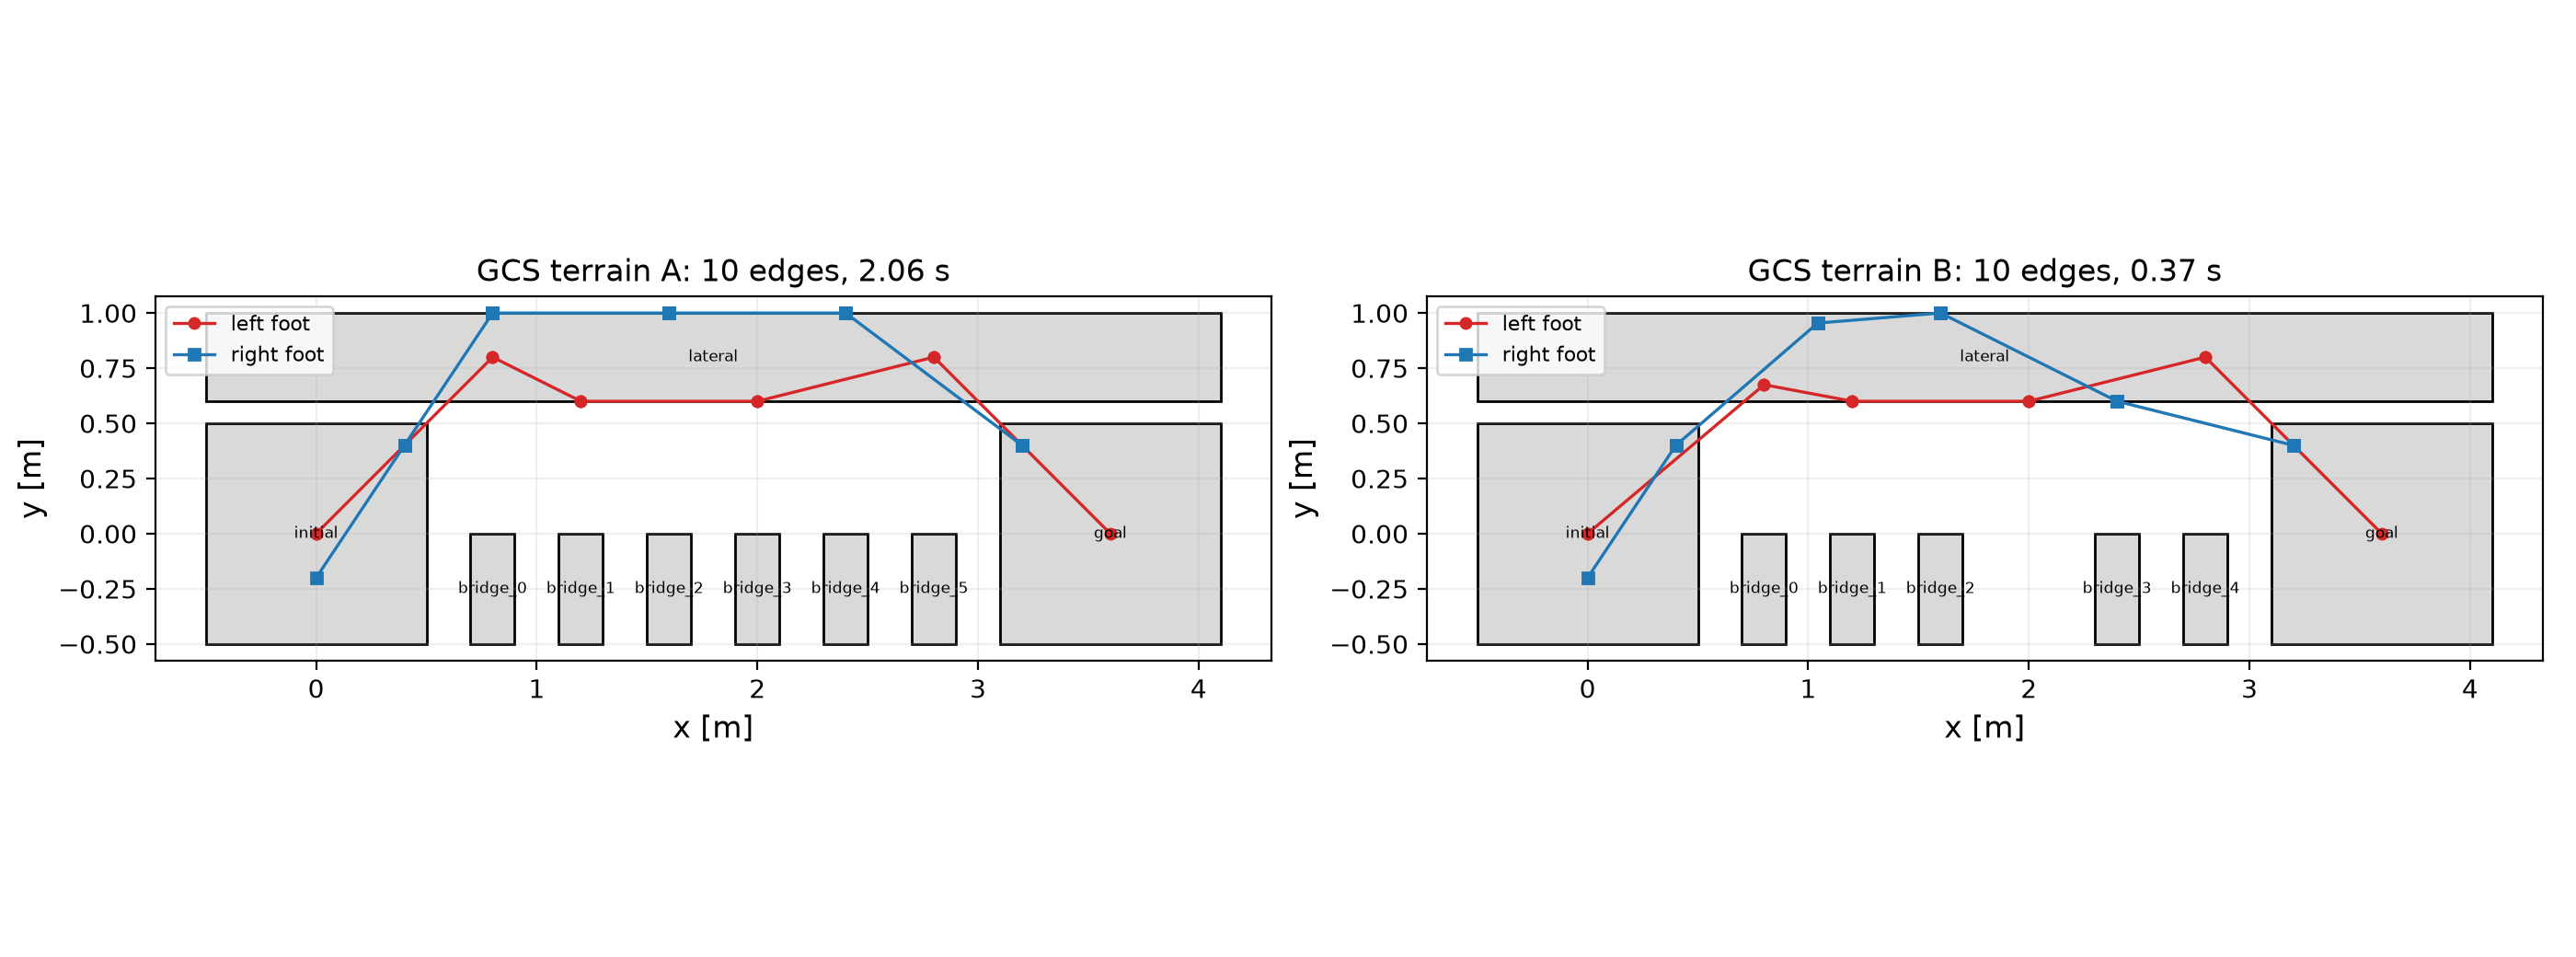
\includegraphics[width=0.98\textwidth]{fig5_5_gcs_plans.png}
  \caption{Section 5.8(c): GCS plans on the six-bridge-stone terrains used in
  the notebook.  Terrain~B detours through the lateral stone, as in the MIQP.}
  \label{fig:gcs_plans}
\end{figure}

\begin{table}[H]
\centering
\caption{Section 5.8(c): GCS results on the notebook terrains
(\texttt{[1,1,1,1,1,1]} and \texttt{[1,1,1,0,1,1]}).}
\begin{tabular}{cccc}
\toprule
Terrain & path cost (edges) & positions & solve time [s] \\
\midrule
A & 10 & 11 & 1.02 \\
B & 10 & 11 & 0.36 \\
\bottomrule
\end{tabular}
\end{table}

The autograder reports
\begin{center}
\textbf{Total score is 16/16: relative position 8/8, objective 8/8.}
\end{center}
The objective checked by the autograder is the squared norm of the summed
displacements, which is not exactly the number-of-steps objective used in the
notebook; the solution passes both because the paths use the same number of
edges and the same geometric route.

\subsection{MIQP versus GCS}

\begin{table}[H]
\centering
\caption{Solving the same bridge terrain with MIQP and GCS.  The MIQP uses
$n_{\rm steps}=n_{\rm bridge}+5$; the GCS has no step limit.  Times are
single-run wall-clock values and exclude model construction.}
\begin{tabular}{cccc}
\toprule
Bridge stones & MIQP time [s] & GCS time [s] & GCS path edges \\
\midrule
4 & 0.96 & 0.39 & 7 \\
6 & 2.23 & 0.44 & 10 \\
8 & 5.00 & 0.77 & 11 \\
\bottomrule
\end{tabular}
\end{table}

\begin{figure}[htbp]
  \centering
  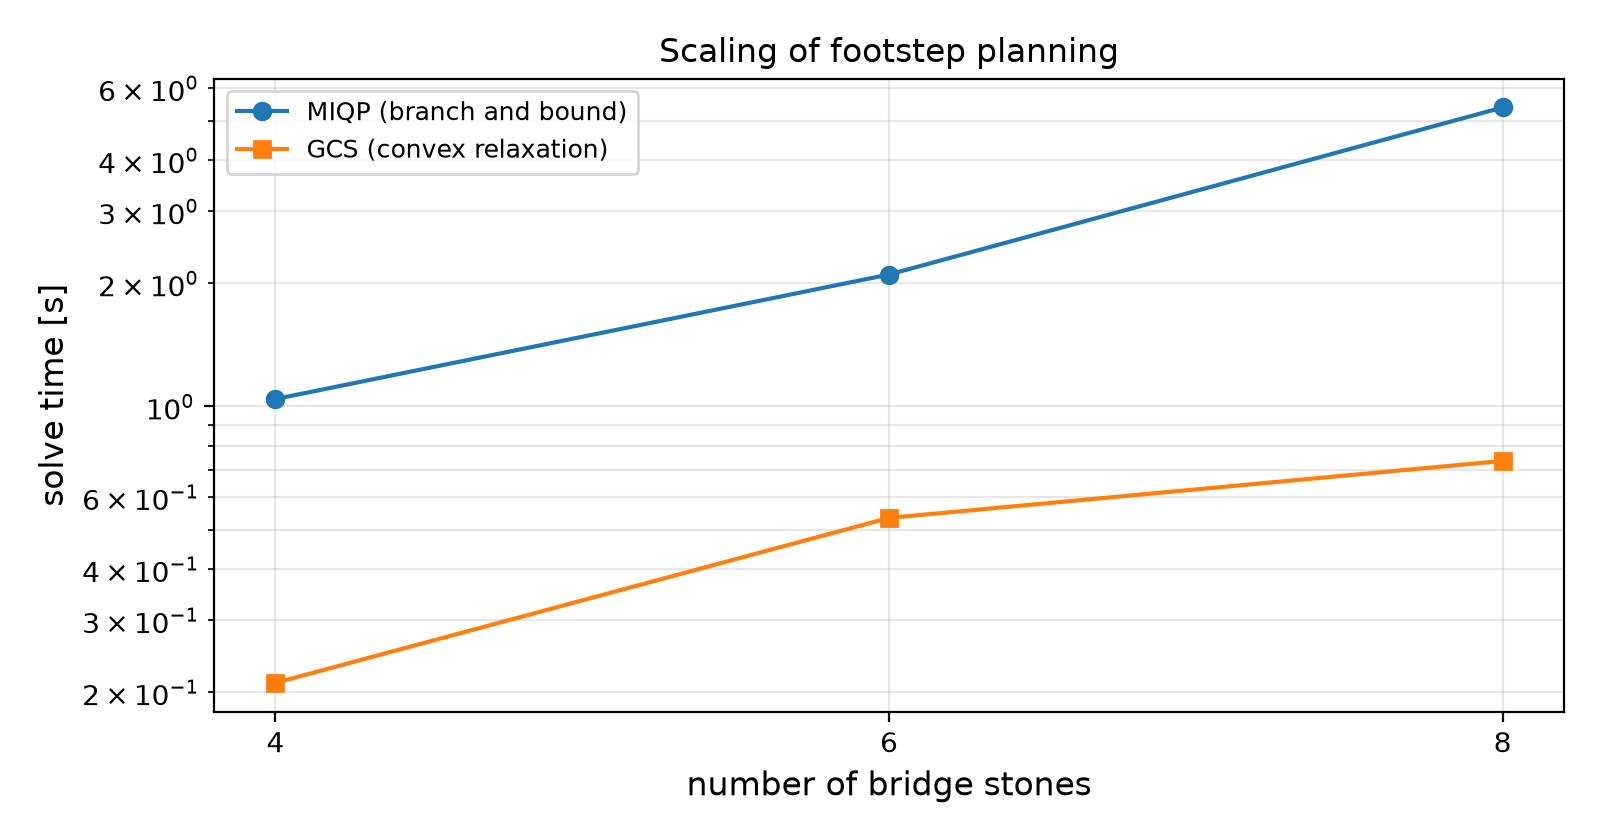
\includegraphics[width=0.75\textwidth]{fig5_7_runtime_scaling.png}
  \caption{Section 5.8(c): solve time versus terrain size.  The MIQP grows
  much faster than the GCS convex relaxation on this range.}
  \label{fig:runtime_scaling}
\end{figure}

\begin{intuition}[breakable=false,title={Why GCS is faster}]
The MIQP has one binary per foot, step and stone; branch and bound must
explore combinations of them.  The GCS encodes the same discrete choice as a
shortest path, and the convex relaxation of the flow variables is a linear
program.  For footstep planning the relaxation is unusually tight, so the
relaxed solution is already integral and no branch and bound is needed.  The
price is that the GCS as implemented here minimizes the number of steps, not
the squared step length; the two objectives coincide on the benchmark terrains
but not in general.
\end{intuition}

\textbf{Comments.}  The GCS is the more scalable formulation, but it requires
careful graph construction: the number of copies, the parent-only entry rule,
and the fixed order of copies.  A naive complete graph would be correct but
much larger; the rules in the exercise keep it sparse.  The MIQP is the more
transparent formulation for teaching because each constraint has a direct
logical meaning.  In practice, the choice depends on the objective and on the
available solver: MIQP with a commercial solver for quadratic step-length
costs, GCS for very large terrains and linear costs.

%=====================================================================
\section{Conclusions}
%=====================================================================

\begin{enumerate}[leftmargin=1.4em]
  \item \textbf{ZMP planning.}  The LIPM turns the CoM/ZMP relation into a
  linear control problem.  Drake's \texttt{ZmpPlanner} returns both a nominal
  CoM trajectory and a feedback policy.  The policy rejects a 0.30~m/s push
  and a 5~cm CoM offset within one 8.5~s footstep plan.  The timing study shows
  the expected trade-off: longer single support means more lateral sway, while
  longer double support means a longer plan but smoother ZMP tracking.
  \item \textbf{LittleDog.}  The gait optimization is a direct transcription
  with exact centroidal dynamics, full kinematics, contact forces and a
  prescribed contact schedule.  SNOPT finds a walking trot in 8.3~s with a
  full stride of 0.6875~s, a 0.25~m stride and a peak foot clearance of
  11.9~mm.  The result is a kinematic/centroidal plan, not a proof of orbital
  stability.
  \item \textbf{MIQP footstep planning.}  The four big-M components (relative
  position, one stone per foot, foot-in-stone, squared step length) solve the
  benchmark terrains to the global optimum and pass 16/16.  The step-span
  sweep shows two thresholds: feasibility at $d=0.8$~m and the lateral-to-
  bridge route switch at $d=1.2$~m.
  \item \textbf{The ZMP exercise.}  Without an ankle actuator the leg is a
  two-force member and the ZMP is the intersection of the leg line with the
  ground, $x_{\rm ZMP}=-h\cot\theta$.  Heel lift occurs when the ZMP reaches
  the toe, $\theta_T=\pi-\arctan(h/L_1)$.  With an ideal ankle actuator the ZMP
  is the CoM projection, $x_{\rm ZMP}=l\cos\theta$, and the posture range is
  narrow for a short foot.  The total foot length dominates the design; $h$
  cancels statically.
  \item \textbf{GCS footstep planning.}  The graph-of-convex-sets transcription
  replaces branch and bound with a shortest path and a tight convex relaxation.
  It passes 16/16 and scales better than the MIQP on the tested terrains
  (0.77~s versus 5.0~s for eight bridge stones).
\end{enumerate}

%=====================================================================
\section{Code and Reproduction}\label{sec:repro}
%=====================================================================

The complete code is in the submission.  Main entry points:
\begin{center}
\small
\begin{tabular}{ll}
\toprule
Topic & Script / notebook \\
\midrule
Example 5.1 & \texttt{Exp5'1-zmp-planner.ipynb}, \texttt{zmp\_analysis.py} \\
Example 5.2 & \texttt{Exp5'2-littledog.ipynb}, \texttt{littledog\_analysis.py} \\
Section 5.8(a) & \texttt{Exp5'8-footstep-planning.ipynb},
\texttt{footstep\_analysis.py} \\
Section 5.8(b) & \texttt{zmp\_exercise\_analysis.py} \\
Section 5.8(c) & \texttt{Exp5'8-footstep-planning-gcs.ipynb},
\texttt{footstep\_analysis.py} \\
\bottomrule
\end{tabular}
\end{center}

Commands (from \texttt{Ch-5/exp5\_analysis}):
\begin{lstlisting}[language=bash]
/Users/leo/venvs/drake/bin/python zmp_analysis.py
/Users/leo/venvs/drake/bin/python littledog_analysis.py
/Users/leo/venvs/drake/bin/python footstep_analysis.py
/Users/leo/venvs/drake/bin/python zmp_exercise_analysis.py
\end{lstlisting}

Headless notebook execution:
\begin{lstlisting}[language=bash]
COLAB_TESTING=1 /Users/leo/venvs/drake/bin/jupyter nbconvert \
  --to notebook --execute --inplace --ExecutePreprocessor.timeout=1200 \
  "Exp5'1-zmp-planner.ipynb"
# The LittleDog notebook must run without COLAB_TESTING so that
# running_as_notebook is true and SNOPT gets its full iteration budget.
/Users/leo/venvs/drake/bin/jupyter nbconvert --to notebook --execute \
  --inplace --ExecutePreprocessor.timeout=3000 "Exp5'2-littledog.ipynb"
\end{lstlisting}

The report is compiled with
\begin{lstlisting}[language=bash]
pdflatex Ch5_Report.tex
pdflatex Ch5_Report.tex
\end{lstlisting}

\appendix
\section{Key Code Snippets}

\subsection{ZMP planner evaluation}

\begin{lstlisting}[language=Python]
def plan_walk(footsteps, double_support_duration, single_support_duration,
              height=1.0, x0=None):
    if x0 is None:
        x0 = np.zeros(4)
    zmp_traj = GenerateDesiredZmpTraj(
        footsteps, double_support_duration, single_support_duration)
    zmp_planner = ZmpPlanner()
    zmp_planner.Plan(zmp_traj, x0, height)
    return zmp_planner, zmp_traj

# Closed-loop rollout with the feedback policy:
for t in ts:
    c = planner.get_nominal_com(t)
    cd = planner.get_nominal_comd(t)
    x = np.concatenate((c, cd))
    cdd = planner.ComputeOptimalCoMdd(t, x)
    zmp = planner.comdd_to_cop(x, cdd)
\end{lstlisting}

\subsection{MIQP constraints}

\begin{lstlisting}[language=Python]
# (a) relative position
for t in range(n_steps + 1):
    relative = position_left[t] - position_right[t]
    prog.AddLinearConstraint(le(relative, step_span / 2))
    prog.AddLinearConstraint(ge(relative, -step_span / 2))

# (b) one stone per foot
for t in range(n_steps + 1):
    prog.AddLinearConstraint(stone_left[t].sum() == 1)
    prog.AddLinearConstraint(stone_right[t].sum() == 1)

# (c) big-M foot-in-stone
for t in range(n_steps + 1):
    for i, stone in enumerate(terrain.stepping_stones):
        prog.AddLinearConstraint(le(
            stone.A.dot(position_left[t]),
            stone.b + (1 - stone_left[t, i]) * M))
        prog.AddLinearConstraint(le(
            stone.A.dot(position_right[t]),
            stone.b + (1 - stone_right[t, i]) * M))

# (d) squared step length
for t in range(n_steps):
    dl = position_left[t + 1] - position_left[t]
    dr = position_right[t + 1] - position_right[t]
    prog.AddQuadraticCost(dl.dot(dl))
    prog.AddQuadraticCost(dr.dot(dr))
\end{lstlisting}

\subsection{GCS edges}

\begin{lstlisting}[language=Python]
def add_vertex_and_edges_for_set_copies(G, T, step_span):
    ...
    def num_copies(stone):
        return int(np.floor(stone.width / step_span)) + 2

def add_edges_towards_parent_vertices(G, V, E_list):
    for u in V:
        if u.name() == "target":
            continue
        u_stem, _ = split_name(u.name())
        for v in V:
            if v.name() == "source":
                continue
            v_stem, v_idx = split_name(v.name())
            if u.name() == "source":
                if v.name() != "target" and v_idx == 0:
                    E_list.append([u, v])
            elif v.name() == "target":
                E_list.append([u, v])
            elif v_stem != u_stem and v_idx == 0:
                E_list.append([u, v])

def add_edge_constraints_costs(G, E_list, step_span):
    for u, v in E_list:
        e = G.AddEdge(u, v)
        for k in range(2):
            e.AddConstraint(e.xu()[k] - e.xv()[k] <= step_span / 2)
            e.AddConstraint(e.xv()[k] - e.xu()[k] <= step_span / 2)
        e.AddCost(1.0)
\end{lstlisting}

\subsection{LittleDog centroidal constraints (sketch)}

\begin{lstlisting}[language=Python]
# CoM Newton-Euler
for n in range(N - 1):
    prog.AddConstraint(eq(com[:, n + 1], com[:, n] + h[n] * comdot[:, n]))
    prog.AddConstraint(eq(comdot[:, n + 1], comdot[:, n] + h[n] * comddot[:, n]))
    prog.AddConstraint(eq(
        total_mass * comddot[:, n],
        sum(contact_force[i][:, n] for i in range(4))
        + total_mass * gravity))

# Angular momentum about the CoM
for n in range(N - 1):
    prog.AddConstraint(eq(H[:, n + 1], H[:, n] + h[n] * Hdot[:, n]))
    prog.AddConstraint(partial(angular_momentum_constraint,
                               context_index=n),
                       lb=np.zeros(3), ub=np.zeros(3),
                       vars=np.concatenate((q[:, n], com[:, n],
                                            Hdot[:, n], Fn)))

# Centroidal consistency: com == CenterOfMass(q),
# H == SpatialMomentumInWorldAboutPoint(q, v, com)
for n in range(N):
    prog.AddConstraint(partial(com_constraint, context_index=n),
                       lb=np.zeros(6), ub=np.zeros(6),
                       vars=np.concatenate((q[:, n], v[:, n],
                                            com[:, n], H[:, n])))
\end{lstlisting}

\end{document}
